%!TEX TS-program = xelatex

\documentclass[c, dvipsnames]{beamer}  % [t], [c], или [b] --- вертикальное 
%\documentclass[handout, dvipsnames, c]{beamer} % Раздаточный материал (на слайдах всё сразу)
% !TEX root = main_file.tex

%%%%%%%%%% Програмный код %%%%%%%%%%
% \usepackage{minted}
% Включает подсветку команд в программах!
% Нужно, чтобы на компе стоял питон, надо поставить пакет Pygments, в котором он сделан, через pip.

% Для Windows: Жмём win+r, вводим cmd, жмём enter. Открывается консоль.
% Прописываем pip install Pygments
% Заходим в настройки texmaker и там прописываем в PdfLatex или XelaTeX:
% pdflatex -shell-escape -synctex=1 -interaction=nonstopmode %.tex

% Для Linux: Открываем консоль. Убеждаемся, что у вас установлен pip командой pip --version
% Если он не установлен, ставим его: sudo apt-get install python-pip
% Ставим пакет sudo pip install Pygments

% Для Mac: Всё то же самое, что на Linux, но через brew.

% После всего этого вы должны почувствовать себя тру-программистами!
% Документация по пакету хорошая. Сам читал, погуглите!

%%%%%%%%%% Математика %%%%%%%%%%
\usepackage{amsmath,amsfonts,amssymb,amsthm,mathtools}
% Показывать номера только у тех формул, на которые есть \eqref{} в тексте.
%\mathtoolsset{showonlyrefs=true}
%\usepackage{leqno} % Нумерация формул слева

%%%%%%%%%% Шрифты %%%%%%%%%%
\usepackage[english, russian]{babel}   % выбор языка для документа
\usepackage[utf8]{inputenc}            % выбор utf8 кодировки
\usepackage[X2,T2A]{fontenc}           % ещё немного кодировки

\usepackage{fontspec}                  % пакет для подгрузки шрифтов
\setmainfont{Times New Roman}          % задаёт основной шрифт документа

\usepackage{unicode-math}              % пакет для установки математического шрифта
\setmathfont{Asana-Math.otf}           % шрифт для математики

% Конкретный символ из конкретного шрифта
% \setmathfont[range=\int]{Neo Euler}

%%%%%%%%%% Работа с картинками %%%%%%%%%%
\usepackage{graphicx}                  % Для вставки рисунков
\usepackage{graphics}
\graphicspath{{images/}{pictures/}}    % можно указать папки с картинками
\usepackage{wrapfig}                   % Обтекание рисунков и таблиц текстом


%%%%%%%%%% Работа с таблицами %%%%%%%%%%
\usepackage{tabularx}            % новые типы колонок
\usepackage{tabulary}            % и ещё новые типы колонок
\usepackage{array,delarray}      % Дополнительная работа с таблицами
\usepackage{longtable}           % Длинные таблицы
\usepackage{multirow}            % Слияние строк в таблице
\usepackage{float}               % возможность позиционировать объекты в нужном месте
\usepackage{booktabs}            % таблицы как в книгах
% Заповеди из документации к booktabs:
% 1. Будь проще! Глазам должно быть комфортно
% 2. Не используйте вертикальные линни
% 3. Не используйте двойные линии. Как правило, достаточно трёх горизонтальных линий
% 4. Единицы измерения - в шапку таблицы
% 5. Не сокращайте .1 вместо 0.1
% 6. Повторяющееся значение повторяйте, а не говорите "то же"
% 7. Есть сомнения? Выравнивай по левому краю!

%  вычисляемые колонки по tabularx
\newcolumntype{C}{>{\centering\arraybackslash}X}
\newcolumntype{L}{>{\raggedright\arraybackslash}X}
\newcolumntype{Y}{>{\arraybackslash}X}
\newcolumntype{Z}{>{\centering\arraybackslash}X}


%%%%%%%%%% Графика и рисование %%%%%%%%%%
\usepackage{tikz, pgfplots}    % язык для рисования графики из latex'a

%%%%%%%%%% Гиперссылки %%%%%%%%%%
\usepackage{xcolor}            % разные цвета

\usepackage{hyperref}
\hypersetup{
    unicode=true,           % позволяет использовать юникодные символы
    colorlinks=true,       	% true - цветные ссылки, false - ссылки в рамках
    urlcolor =blue,         % цвет ссылки на url
    linkcolor=black,        % внутренние ссылки
    citecolor=black,        % на библиографию
	breaklinks              % если ссылка не умещается в одну строку, разбивать ли ее на две части?
}

%%%%%%%%%% Другие приятные пакеты %%%%%%%%%%
\usepackage{multicol}       % несколько колонок
\usepackage{verbatim}       % для многострочных комментариев
\usepackage{enumitem}       % дополнительные плюшки для списков
%  например \begin{enumerate}[resume] позволяет продолжить нумерацию в новом списке

\usepackage{todonotes}      % для вставки в документ заметок о том, что  осталось сделать
% \todo{Здесь надо коэффициенты исправить}
% \missingfigure{Здесь будет Последний день Помпеи}
% \listoftodos --- печатает все поставленные \todo'шки

%%%%%%%%%%%%%%%%%%%%%%%%%%%%%%%%%%%%%%%%%%%
%%%%%%%%%% ГОСТОВСКИЕ ПРИБАМБАСЫ %%%%%%%%%%
%%%%%%%%%%%%%%%%%%%%%%%%%%%%%%%%%%%%%%%%%%%

% размер листа бумаги
\usepackage[paper=a4paper,top=15mm, bottom=15mm,left=35mm,right=10mm,includehead]{geometry}

% всякие разные расстояния
\usepackage{setspace}
\setstretch{1.33}              % Полуторный межстрочный интервал
\setlength{\parindent}{1.5em}  % Красная строка.

\righthyphenmin=2    % Разрешение переноса двух и более символов
\widowpenalty=10000  % Наказание за вдовствующую строку (одна строка абзаца на этой странице, остальное --- на следующей)
%\clubpenalty=10000  % Наказание за сиротствующую строку (омерзительно висящая одинокая строка в начале страницы)
\tolerance=1000      % Ещё какое-то наказание.

% Нумерация страниц сверху по центру
\usepackage{fancyhdr}
\pagestyle{fancy}
\fancyhead{ } % clear all fields
\fancyfoot{ } % clear all fields
\fancyhead[C]{\thepage}
% Чтобы не прорисовывалась черта!
\renewcommand{\headrulewidth}{0pt}

% Нумерация страниц с надписью "Глава"
\usepackage{etoolbox}
\patchcmd{\chapter}{\thispagestyle{plain}}{\thispagestyle{fancy}}{}{}

% Заголовки по левому краю
% опция identfirst устанавливает отступ в первом абзаце
\usepackage[indentfirst]{titlesec}{\raggedleft}

% В Linux этот пакет для заголовков. Исправляет это следующий непонятный кусок кода:
\makeatletter
\patchcmd{\ttlh@hang}{\parindent\z@}{\parindent\z@\leavevmode}{}{}
\patchcmd{\ttlh@hang}{\noindent}{}{}{}
\makeatother

% Редактирования Глав и названий
\titleformat{\chapter}
      {\normalfont\large\bfseries}
      {\thechapter }{0.5 em}{}

% Редактирование ненумеруемых глав chapter* (Введение и тп)
\titleformat{name=\chapter,numberless}
{\centering\normalfont\bfseries\large}{}{0.25em}{\normalfont}

% Убирает чеканутые отступы вверху страницы
\titlespacing{\chapter}{0pt}{-\baselineskip}{\baselineskip}

% Более низкие уровни (подзаголовки)
\titleformat{\section}{\bfseries}{\thesection}{0.5 em}{}
\titleformat{\subsection}{\bfseries}{\thesubsection}{0.5 em}{}

\titlespacing*{\section}{0 pt}{\baselineskip}{\baselineskip}
\titlespacing*{\subsection}{0 pt}{\baselineskip}{\baselineskip}

% Содержание, команды ниже изменяют отступы и рисуют точечки!
\usepackage{titletoc}

\titlecontents{chapter}
             [1em] %
             {\normalsize}
             {\contentslabel{1 em}}
             {\hspace{-1 em}}
             {\normalsize\titlerule*[10pt]{.}\contentspage}

\titlecontents{section}
              [3 em] %
              {\normalsize}
              {\contentslabel{1.75 em}}
              {\hspace{-1.75 em}}
              {\normalsize\titlerule*[10pt]{.}\contentspage}

\titlecontents{subsection}
              [6 em] %
              {\normalsize}
              {\contentslabel{3 em}}
              {\hspace{-3 em}}
              {\normalsize\titlerule*[10pt]{.}\contentspage}

% Правильные подписи под таблицей и рисунком
% Документация к пакету на русском языке!
\usepackage[tableposition=top, singlelinecheck=false]{caption}
\usepackage{subcaption}

   \DeclareCaptionStyle{base}%
		[justification=centering,indention=0pt]{}
   \DeclareCaptionLabelFormat{gostfigure}{Рисунок #2}
   \DeclareCaptionLabelFormat{gosttable}{Таблица #2}

   \DeclareCaptionLabelSeparator{gost}{~---~}
   \captionsetup{labelsep=gost}

   \DeclareCaptionStyle{fig01}%
           [margin=5mm,justification=centering]%
           {margin={3em,3em}}
   \captionsetup*[figure]{style=fig01,labelsep=gost,labelformat=gostfigure,format=hang}

   \DeclareCaptionStyle{tab01}%
           [margin=5mm,justification=centering]%
           {margin={3em,3em}}
   \captionsetup*[table]{style=tab01,labelsep=gost,labelformat=gosttable,format=hang}

% межстрочный отступ в таблице
 \renewcommand{\arraystretch}{1.2}

% многостраничные таблицы под РОССИЙСКИЙ СТАНДАРТ
% ВНИМАНИЕ! Обязательно после пакета caption!
\usepackage{fr-longtable}

%Более гибкие спсики
\usepackage{enumitem}

% сообщаем окружению о том, что существует такая штука, как нумерация русскими буквами
\makeatletter
\AddEnumerateCounter{\asbuk}{\russian@alph}{щ}
\makeatother

% ГОСТОВСКИЕ СПИСКИ

% Первый тип списков. Большая буква.
\newlist{Enumerate}{enumerate}{1}

\setlist[Enumerate,1]{labelsep=0.5em,leftmargin=1.25em,labelwidth=1.25em,
parsep=0em,itemsep=0em,topsep=0ex, before={\parskip=-1em},label=\arabic{Enumeratei}.}

% Второй тип списков. Маленькая буква.
\setlist[enumerate]{label=\arabic{enumi}),parsep=0em,itemsep=0em,topsep=0.75ex, before={\parskip=-1em}}

% Третий тип списков. Два уровня.
\newlist{twoenumerate}{enumerate}{2}
\setlist[twoenumerate,1]{itemsep=0mm,parsep=0em,topsep=0.75ex,, before={\parskip=-1em},label=\asbuk{twoenumeratei})}
\setlist[twoenumerate,2]{leftmargin=1.3em,itemsep=0mm,parsep=0em,topsep=0ex, before={\parskip=-1em},label=\arabic{twoenumerateii})}

% Четвёртый тип списков. Список с тире.
\setlist[itemize]{label=--,parsep=0em,itemsep=0em,topsep=0ex, before={\parskip=-1em},after={\parskip=-1em}}

% WARNING WARNING WARNIN!
% Если в списке предложения, то должна по госту стоять точка после цифры => команда Enumerate! Если идет перечень маленьких фактов, не обособляемых предложений то после цифры идет скобка ")" => команда enumerate! Если перечень при этом ещё и двууровневый, то twoenumerate.


%%%%%%%%%% Список литературы %%%%%%%%%%

%\usepackage[
%backend=biber, %подключение пакета biber (тоже нужен)
%bibstyle=gost-numeric, %подключение одного из четырех главных стилей biblatex-gost
%sorting=ntvy, %тип сортировки в библиографии
%]{biblatex}
\usepackage[backend=biber,style=gost-numeric, maxbibnames=9,maxcitenames=2,uniquelist=false, babel=other]{biblatex}

% Справка по 4 главным стилям для ленивых:
% gost-inline  ссылки внутри теста в круглых скобках
% gost-footnote подстрочные ссылки
% gost-numeric затекстовые ссылки
% gost-authoryear тоже затекстовые ссылки, но немного другие

% Подробнее смотри страницу 4 документации. Она на русском.

% Ещё немного настроек
\DeclareFieldFormat{postnote}{#1} %убирает с. и p.
\renewcommand*{\mkgostheading}[1]{#1} % только лишь убираем курсив с авторов

\addbibresource{bib.bib} 

% Этот кусок кода выносит русские источники на первое место. Костыль описали авторы пакета в руководстве к нему. Подробнее смотри:
% https://github.com/odomanov/biblatex-gost/wiki/Как-сделать%2C-чтобы-русскоязычные-источники-предшествовали-остальным
\DeclareSourcemap{
  \maps[datatype=bibtex]{
    \map{
      \step[fieldsource=langid, match=russian, final]
      \step[fieldset=presort, fieldvalue={a}]
    }
    \map{
      \step[fieldsource=langid, notmatch=russian, final]
      \step[fieldset=presort, fieldvalue={z}]
    }
  }
}

\DefineBibliographyStrings{english}{%
pages = {P\adddot},
number = {№},
}

\title[]{Прогнозирование и оценка макроэкономических зависимостей при помощи методов снижения размерности в данных на примере инвестиций в России}


\author[Михаил Гареев]{Михаил Гареев \\ \smallskip \scriptsize ЭО-15-01 \\ \smallskip \scriptsize \href{mailto:mkhlgrv@gmail.com}{\nolinkurl{mkhlgrv@gmail.com} }}

\superviser{к.э.н. Полбин А.В.}

\institute[РАНХиГС]{ \uppercase{
  Российская Академия Народного Хозяйства и  \\ Государственной Службы при Президенте Российской Федерации}}
\date{2019}


\titlegraphic{
\includegraphics[scale=0.5]{logo/logo_ranepa.png}}
\titlegraphicii{
\includegraphics[scale=0.5]{logo/logo_emit.png}}

\begin{document}

\frame[plain]{\titlepage}	% Титульный слайд


\begin{frame}[c]{Актуальность исследования} 
\begin{itemize}
\item  В последнее время методы снижения размерности активно исследуются на возможность прогнозирования макроэкономических данных в России. 
\item Основная идея таких методов --- это некоторый автоматический отбор объясняющих переменных из обширного списка предикторов. 
\item Интересно применить такой подход к оцениванию и прогнозированию уровня инвестиций в России и сравнить его с обычными моделями.
\end{itemize}
\end{frame}





\section{Анализ предметной области}
\begin{frame}[shrink = 40]
 \frametitle{\insertsection} 

\begin{table}[ht]
\centering
\begin{tabular}{llll}
  \hline
Авторы, год & Название & Источник & Результат  \\ 
  \hline
Clark J. M. & Business acceleration & Journal of & Оптимальный уровень капитала прямо \\
(1917) & and  the law of demand: & political&   пропорционален выпуску, и при\\
& A technical factor  & economy  & изменении последнего фирмы мгновенно \\
&in economic cycles  & &  подстраивают уровень капитала \\
& & & под оптимальный через инвестиции\\
\hline
Koyck, L. M.  & Distributed lags  & North-Holland & Подстройка под оптимальный уровень\\
(1954)& and investment analysis & Publishing  &  происходит не мгновенно, а с лагами\\
& &   Company & \\
\hline
Jorgenson &  Capital theory & The American & Уровень инвестиций определяется\\
D.W. (1963)  & and investment behavior  &Economic Review  & издержками использования капитала\\
\hline

Tobin, J. &  A general equilibrium & Journal of money & Чистые инвестиции определяются отношением \\
(1969) &  approach  & credit and banking& рыночной стоимости фирм\\
&
to monetary theory
&
&
и ее амортизационной стоимостью
\\
\hline 
&
&
&
\\
\hline
Belloni, A., & High dimensional  & Bernoulli & Методы регуляризации применены \\
Chernozhukov, V.&  sparse econometric & &для проверки гипотезы конвергенции \\
(2013)
&  models: An introduction
& 
&
\\

\hline

Байбуза, И.  & Прогнозирование  & Деньги и кредит & Методы снижения размерности \\
(2018)
&
инфляции помощью
&
&
и машинного обучения при некоторых условиях\\
&
методов машинного
&
&
превосходят традиционные бенчмарки \\
& обучения
&
& в предсказании месячной \\
&
&
&
инфляции в России \\



   
\end{tabular}
\end{table}
\end{frame}

\begin{frame}[shrink=3]
	\frametitle{Цели и задачи}
	\begin{block}{Цель:}
	\begin{itemize}
		\item Проверка целесообразности использования методов снижения размерности в данных при оценке и прогнозировании российских макроэкономических показателей на примере инвестиций.
	\end{itemize}
		
	\end{block}

	 	\begin{block}{Задачи:}
			\begin{enumerate}
			\item Обзор традиционных методов оценки и прогнозирования инвестиций (акселераторная модель, неоклассическая модель, модель $q$ Тобина, модель авторегрессии);
	\item Обзор методов снижения размерности и машинного обучения (LASSO, Post-LASSO, Ridge, Elastic Net, Random Forest, Spike-and-Slab);
    \item Применение этих методов для прогнозирования уровня инвестиций в России, анализ результатов, сравнение с традиционными методами прогнозирования инвестиций и с результатами использования этих методов.
	 \end{enumerate}	
	\end{block}
\end{frame}


\section{Гипотезы}
\begin{frame}[с, shrink=5]
\frametitle{\insertsection} 

\begin{enumerate}
	\item Использование методов снижения размерности и машинного обучения позволит улучшить качество прогнозов инвестиций в России;
	\item При помощи методов снижения размеhности можно выявить опережающие индикаторы уровня инвестиций.
	 \end{enumerate}

\begin{center}

\end{center}


\end{frame}

\section{Традиционные модели}


\section{Методы снижения размерности}


\subsection{Регуляризация}



\begin{frame}
\frametitle{\insertsection} 
\framesubtitle{\insertsubsection}

 \begin{block}{LASSO}
  \begin{equation}
  \hat{\beta}^{\text{LASSO}} \in \arg \min_{\beta \in
\mathbb{R}^p} \sum_{i=1}^n \left[ (y_i - {x_i}^{'} \beta)^2 \right] +  \frac{\lambda}{n} \left\lVert \beta \right\rVert_1,
\end{equation}
где $\lambda$ --- параметр штрафа.
 \end{block}
  \begin{block}{Ridge}
  \begin{equation}
  \hat{\beta}^{\text{Ridge}} \in \arg \min_{\beta \in
\mathbb{R}^p} \sum_{i=1}^n \left[ (y_i - {x_i}^{'} \beta)^2 \right] +  \frac{\lambda}{n} \left\lVert \beta \right\rVert_2,
\end{equation}
где $\lambda$ --- параметр штрафа.
 \end{block}
 
  \end{frame}

\begin{frame}[shink=20]
\frametitle{\insertsection} 
\framesubtitle{\insertsubsection}
\begin{block}{Post-LASSO}
\begin{enumerate}
    \item Используя метод LASSO, найти $\hat{\beta}^{\text{LASSO}}$,
    \item Применить МНК-регрессию, оценивая только неисключенные элементы $\hat{\beta}^{\text{LASSO}}$:
    \begin{equation}
  \hat{\beta}^{\text{Post-LASSO}} \in \arg \min_{\beta \in
\mathbb{R}^p} \sum_{i=1}^n \left[ (y_i - {x_i}^{'} \beta)^2 \right] \text{,  где }  \beta_j = 0 \text{, если } \hat{\beta_j} = 0.
\end{equation}
\end{enumerate}
\end{block}


\begin{block}{Adaptive LASSO}
\begin{itemize}
    \item Функция штрафа умножается на веса $w$:
     \begin{equation}
  \hat{\beta}^{\text{LASSO}} \in \arg \min_{\beta \in
\mathbb{R}^p} \sum_{i=1}^n \left[ (y_i - {x_i}^{'} \beta)^2 \right] +  \frac{\lambda}{n} w \left\lVert \beta \right\rVert_1,
\end{equation}
\item Веса могут определяться, например, через коэффиценты $\hat{\beta}^{Ridge}$ в Ridge-регрессии:
\begin{equation}
    w_i = \frac{1}{\left(|\hat{\beta}^{Ridge}|\right)^{\gamma}},
\end{equation}
\end{itemize}
\end{block}
\end{frame}

\begin{frame}
\frametitle{\insertsection} 
\begin{block}{Случайный лес}
    Двухэтапное получение оценок:
    \begin{enumerate}
        \item На разных подвыборках данных строится множество решающих деревьев,
        \item В качестве предсказанного значения $\hat{y_i}$ выбираются усреднённые значения показаний по всем деревьям.
    \end{enumerate}
\end{block}

\begin{block}{Регрессия пик-плато (Spike-and-slab)}

    \begin{itemize}
        \item $\beta_j|\tau_j, r^2_j \sim N(0,\tau_j\cdot r^2_j )$
        \item \begin{equation}
             \tau_j = 
 \begin{cases}
   0 &\text{se $\omega\in A$}\\
   1 &\text{se $\omega \in A^c$}
 \end{cases}
        \end{equation}
        \item $r^2_j \sim \text{Exp}(\lambda)$ 
    \end{itemize}
    
    
\end{block}


\end{frame}

\section{Прогнозирование инвестиций}
\subsection{Описание данных и методология}
\begin{frame}[shrink=10]
\frametitle{\insertsection} 
\framesubtitle{\insertsubsection}
\begin{block}{Данные}
\begin{itemize}
        \item Прогнозируемая переменная: валовые инвестиции в основной капитал в России в постоянных ценах, индекс (квартальные данные, 2001.I -- 2018.IV),
    \item Объясняющие переменные: ряды данных, отражающих различные макроэкономические показатели в России (квартальные данные, 2001.I -- 2018.IV).
\end{itemize}
\end{block}
\begin{block}{Схема прогноза}
Модели обучаются на тренировочной выборке (2000.I -- 2014.IV), после чего строится статический прогноз на тестовой выборке (2015.I -- 2018.IV).
\end{block}




\begin{block}{Метрика качества}
Основная метрика качества моделей --- RMSE (root-mean-square error):
\begin{equation}
   \text{RMSE} = \sqrt{ \frac{\sum_{t = 1}^{n} (\hat{y_t} - y_t)}{n}} 
\end{equation}
\end{block}

\end{frame}

 \begin{frame}
\frametitle{\insertsection} 
\begin{figure*}
\caption{Реальные инвестиции в России}
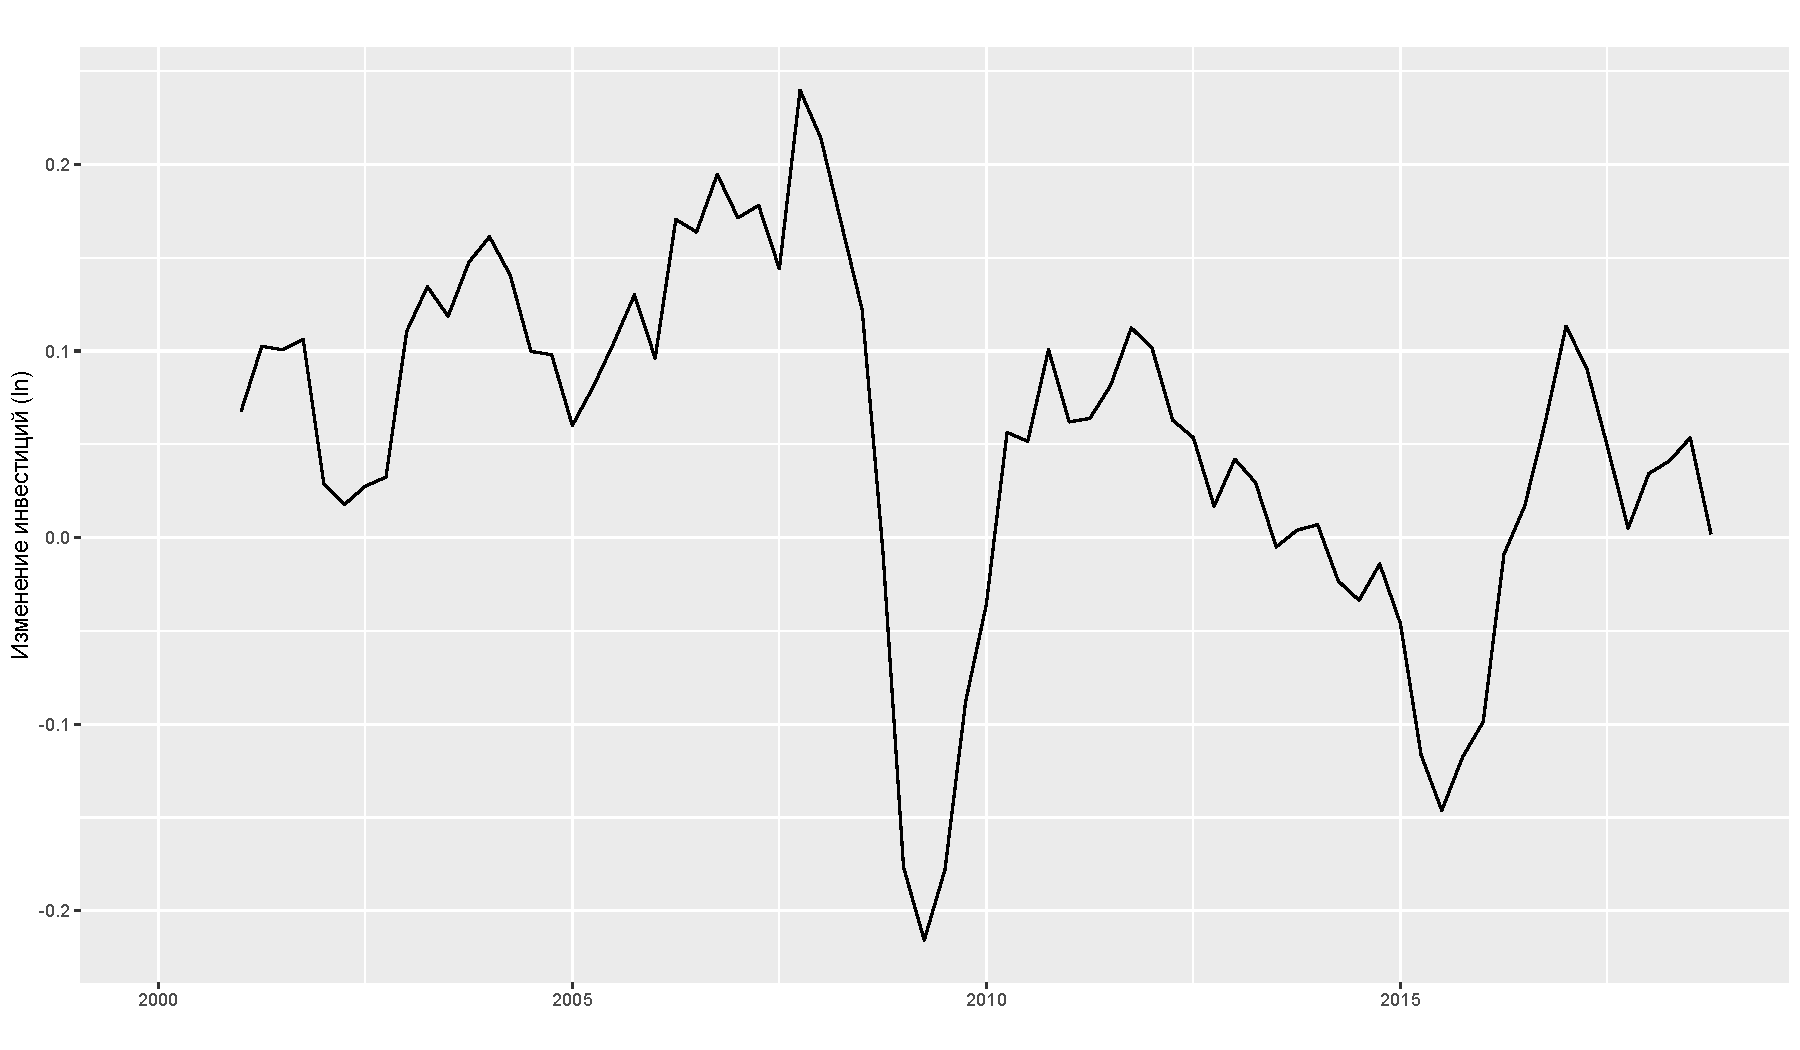
\includegraphics[width=\linewidth]{lineplot2.pdf}
\end{figure*}
\end{frame} 

\subsection{Результаты}
 
 \begin{frame}
 \frametitle{\insertsection} 
\framesubtitle{\insertsubsection}
\begin{table}[ht]
\centering
\begin{tabular}{lrr}
  \hline
Модель & RMSE & R^2  \\ 
  \hline
  Акселератор & 0.057 & 0.44 \\
  Неоклассическая & 0.058 & 0.44 \\
  q Тобина & 0.049 & 0.60 \\
  AR(p) & \alert{0.038} & \alert{0.65} \\
  \hline
  LASSO & 0.044 & 0.67 \\
  Ridge & 0.056 & 0.46 \\
  Adaptive LASSO & 0.088 & -0.32 \\
  Post-LASSO & 0.045 &  0.65 \\
  \hline
  LASSO + неоклассическая & 0.051 & 0.56 \\
  LASSO + q Тобина & 0.043 &0.65 \\
  LASSO + AR(p) & 0.040 & 0.65 \\
   \hline 
   Случайный лес & 0.041 & 0.65 \\
   Пик-плато &0.045 & 0.66 \\
   \hline 
\end{tabular}
\end{table}
\end{frame}

 \begin{frame}
\frametitle{\insertsection} 
\framesubtitle{\insertsubsection}
\begin{figure*}
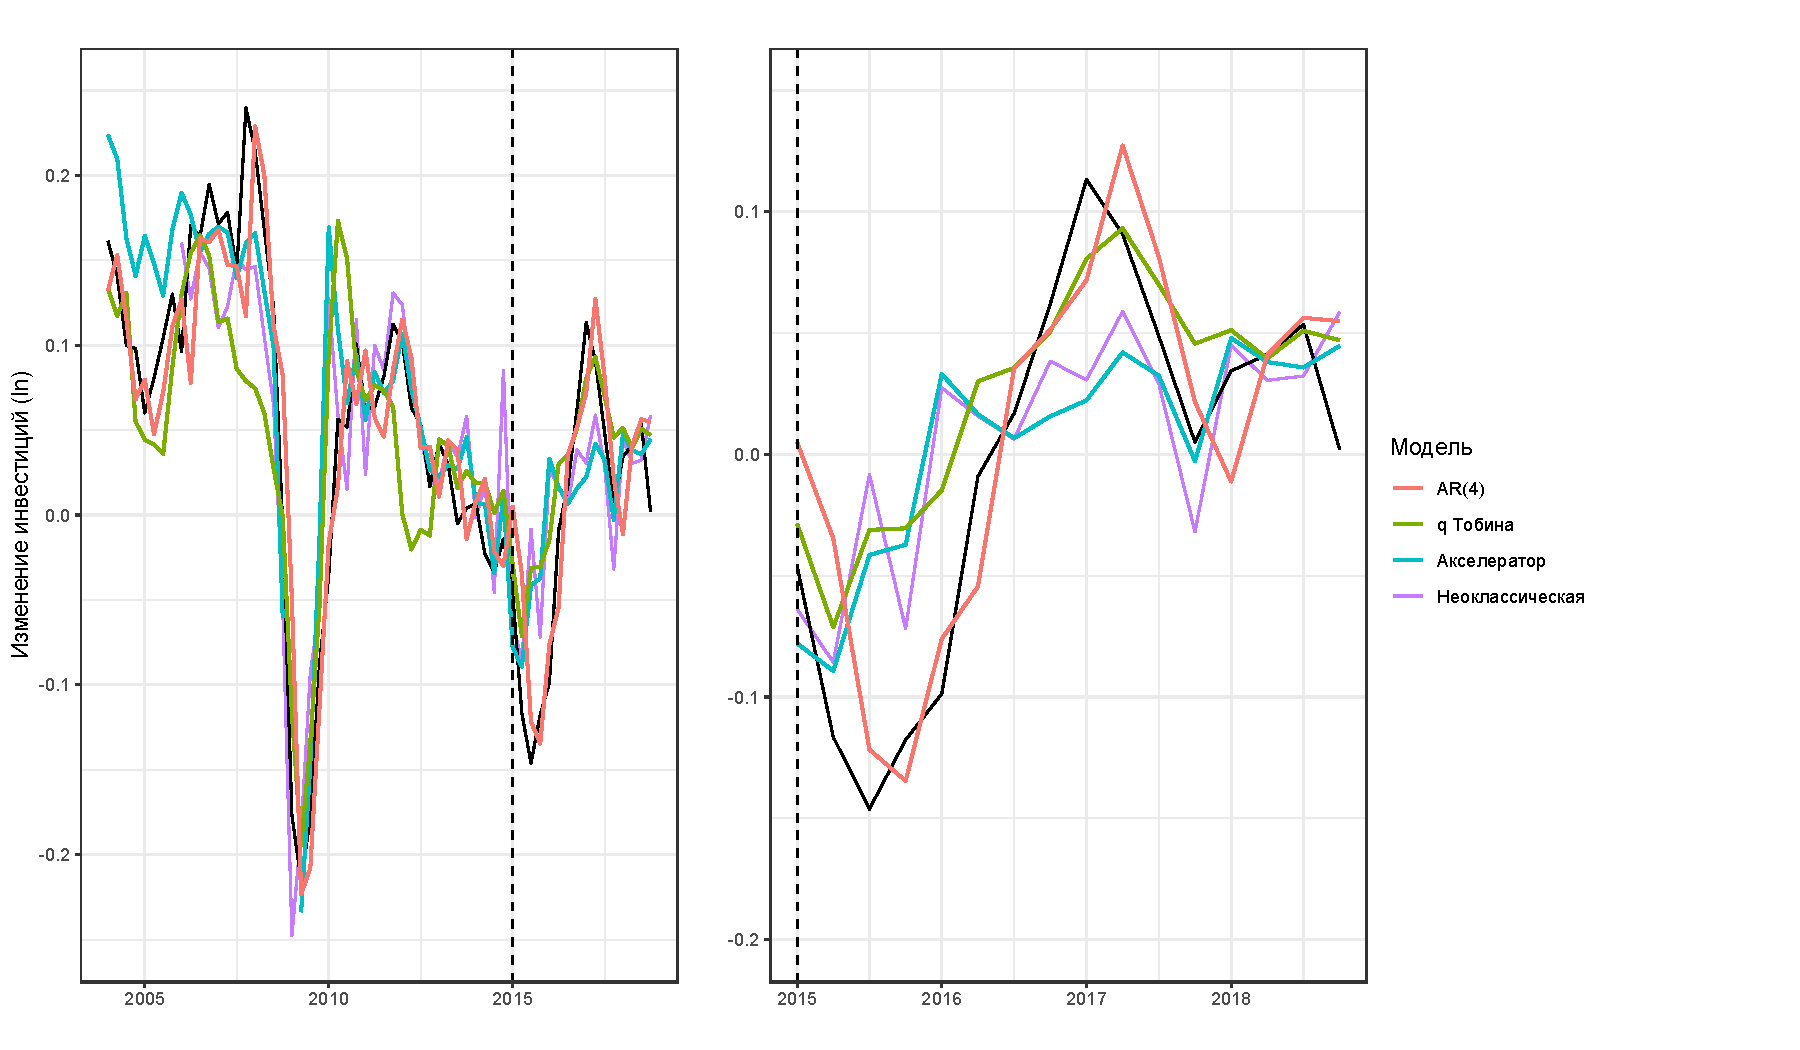
\includegraphics[width=\linewidth]{lineplot1.pdf}
\end{figure*}
\end{frame} 

 \begin{frame}
\frametitle{\insertsection} 
\framesubtitle{\insertsubsection}
\begin{figure*}
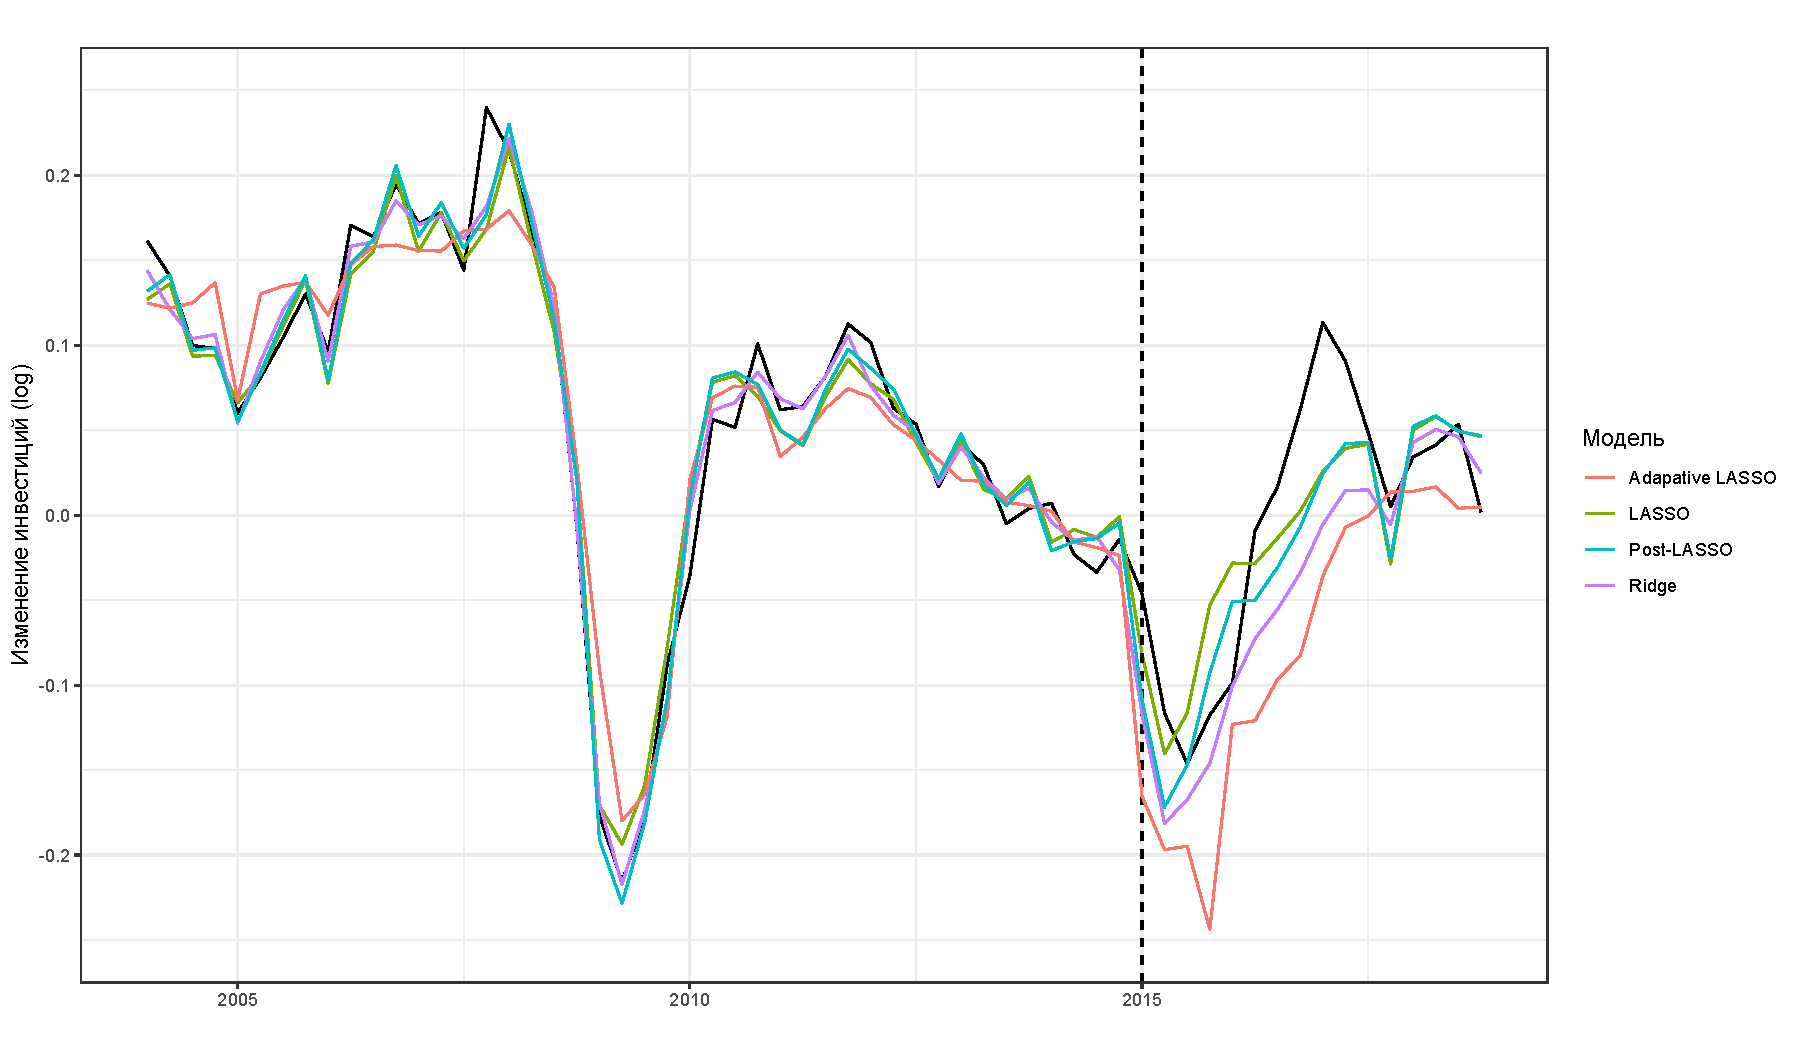
\includegraphics[width=\linewidth]{regular_plot.pdf}
\end{figure*}
\end{frame} 


 \begin{frame}
\frametitle{\insertsection} 
\framesubtitle{\insertsubsection}
\begin{figure*}
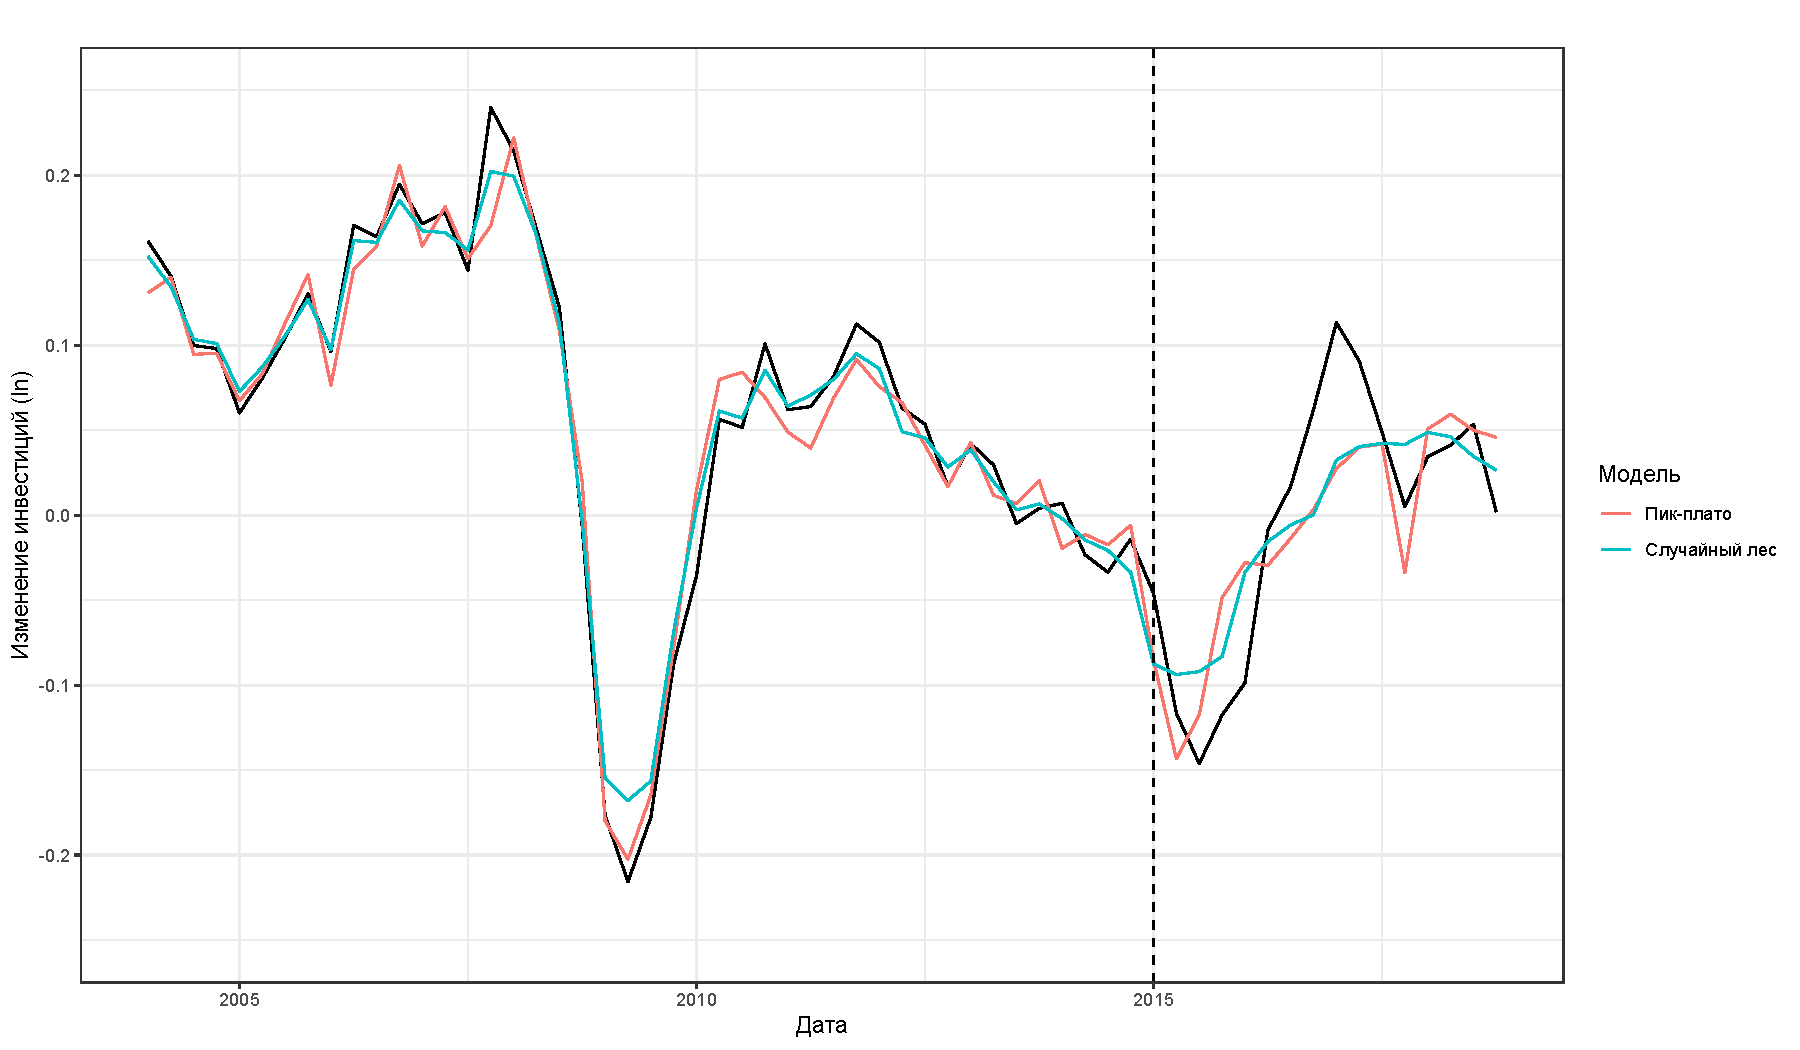
\includegraphics[width=\linewidth]{add_plot.pdf}
\end{figure*}
\end{frame} 


 \begin{frame}
\frametitle{\insertsection} 
\framesubtitle{\insertsubsection}
\begin{figure*}
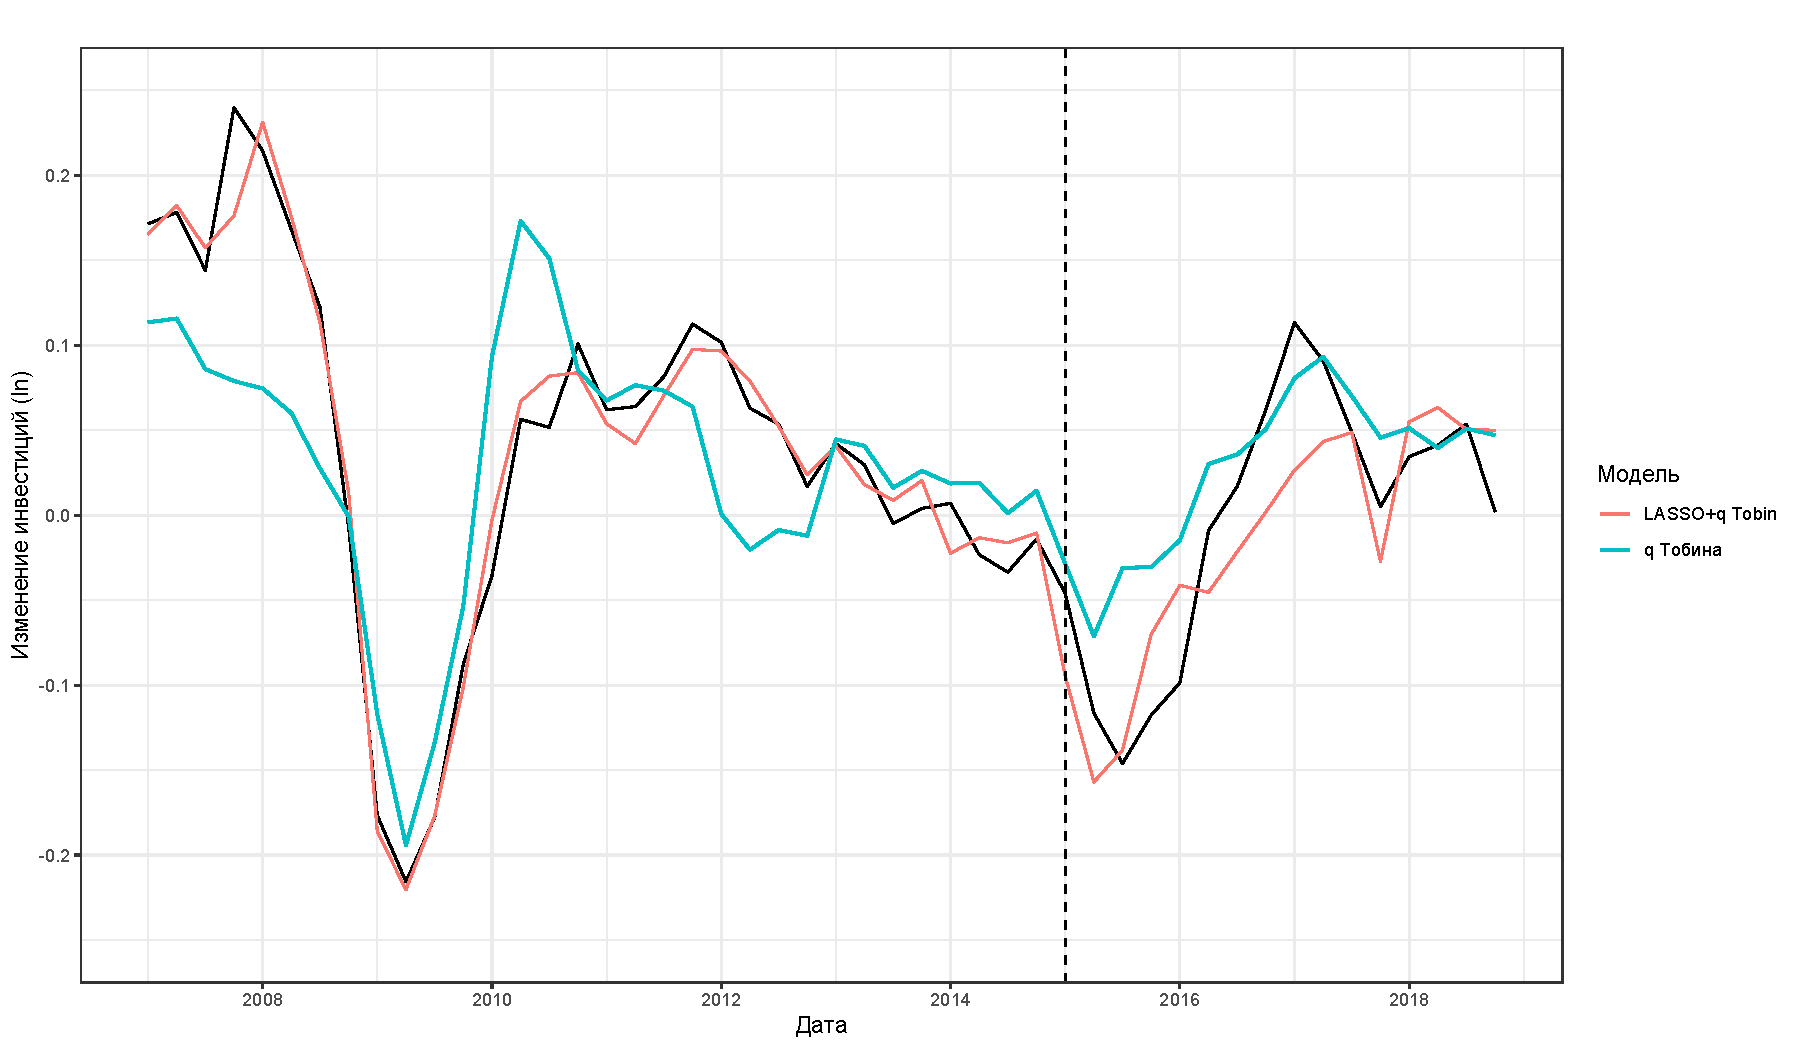
\includegraphics[width=\linewidth]{lq_plot.pdf}
\end{figure*}
\end{frame} 


 \begin{frame}
\frametitle{\insertsection} 
\framesubtitle{\insertsubsection}
\begin{figure*}
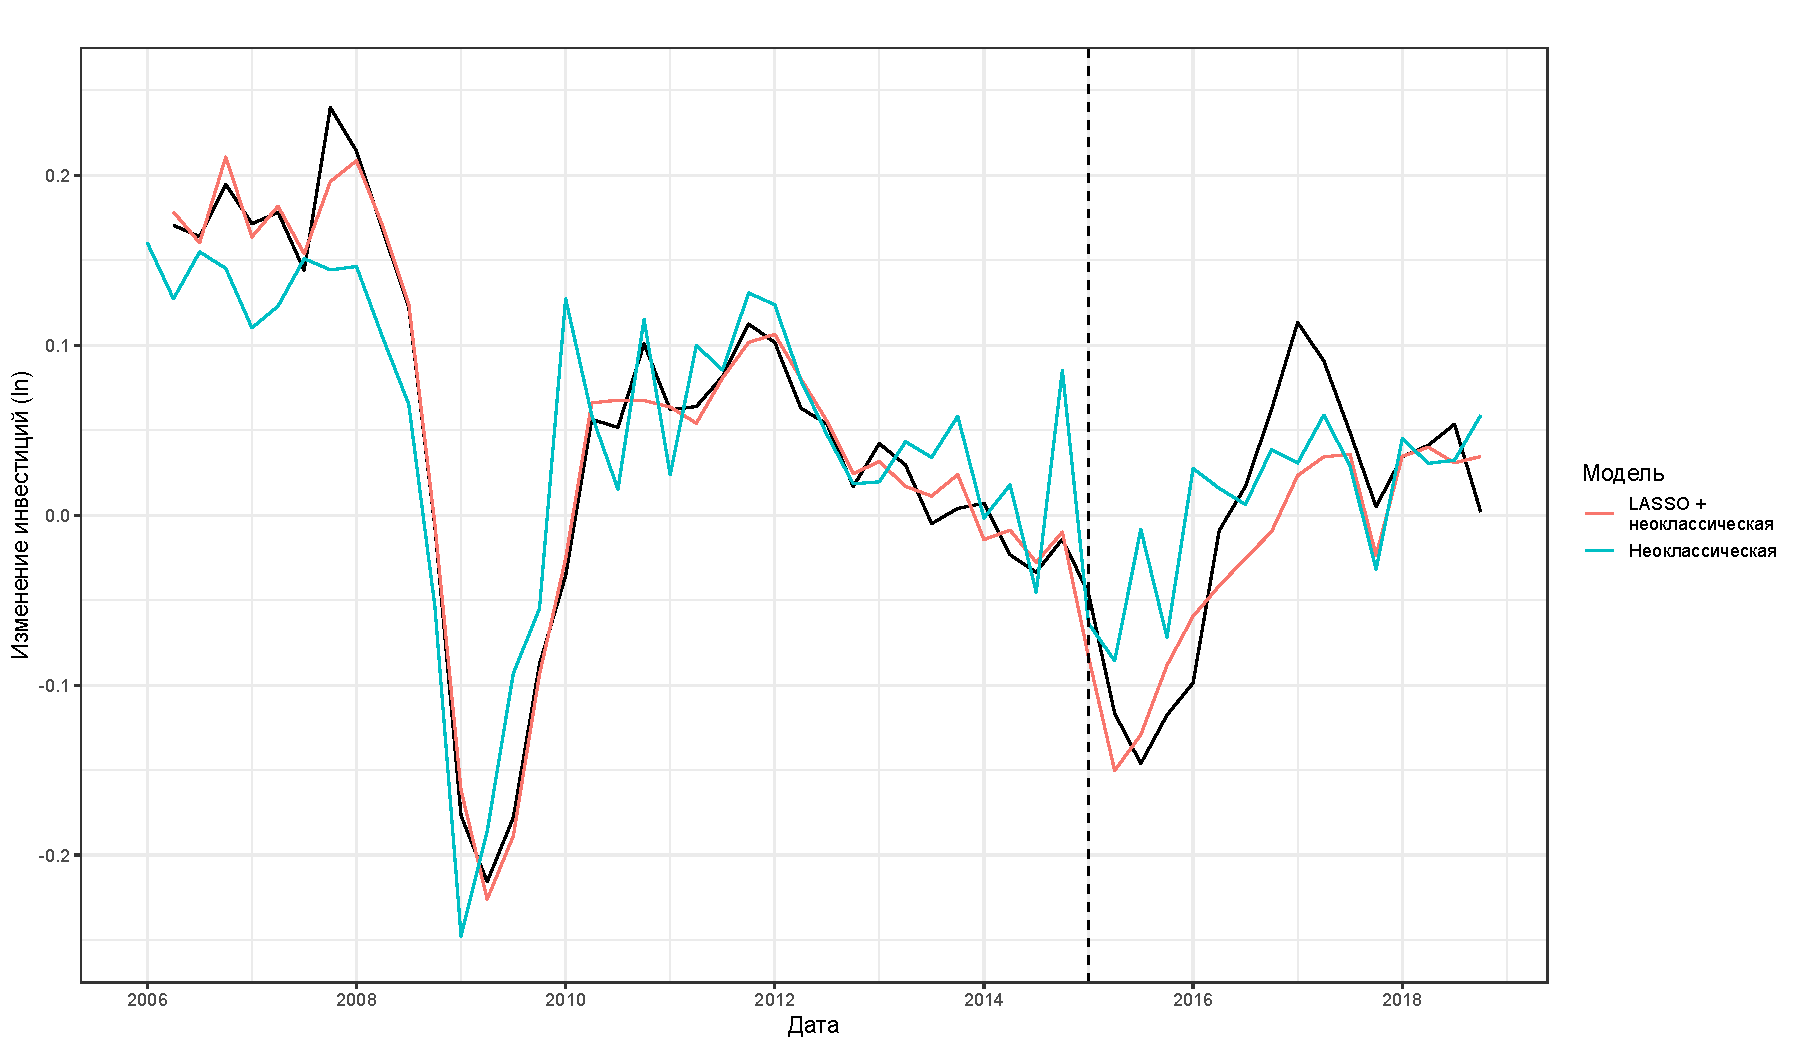
\includegraphics[width=\linewidth]{lnc_plot.pdf}
\end{figure*}
\end{frame} 

\begin{frame}
\frametitle{\insertsection} 
\framesubtitle{\insertsubsection} 
\begin{figure*}
\caption{Апостериорная вероятность значимости регрессоров}
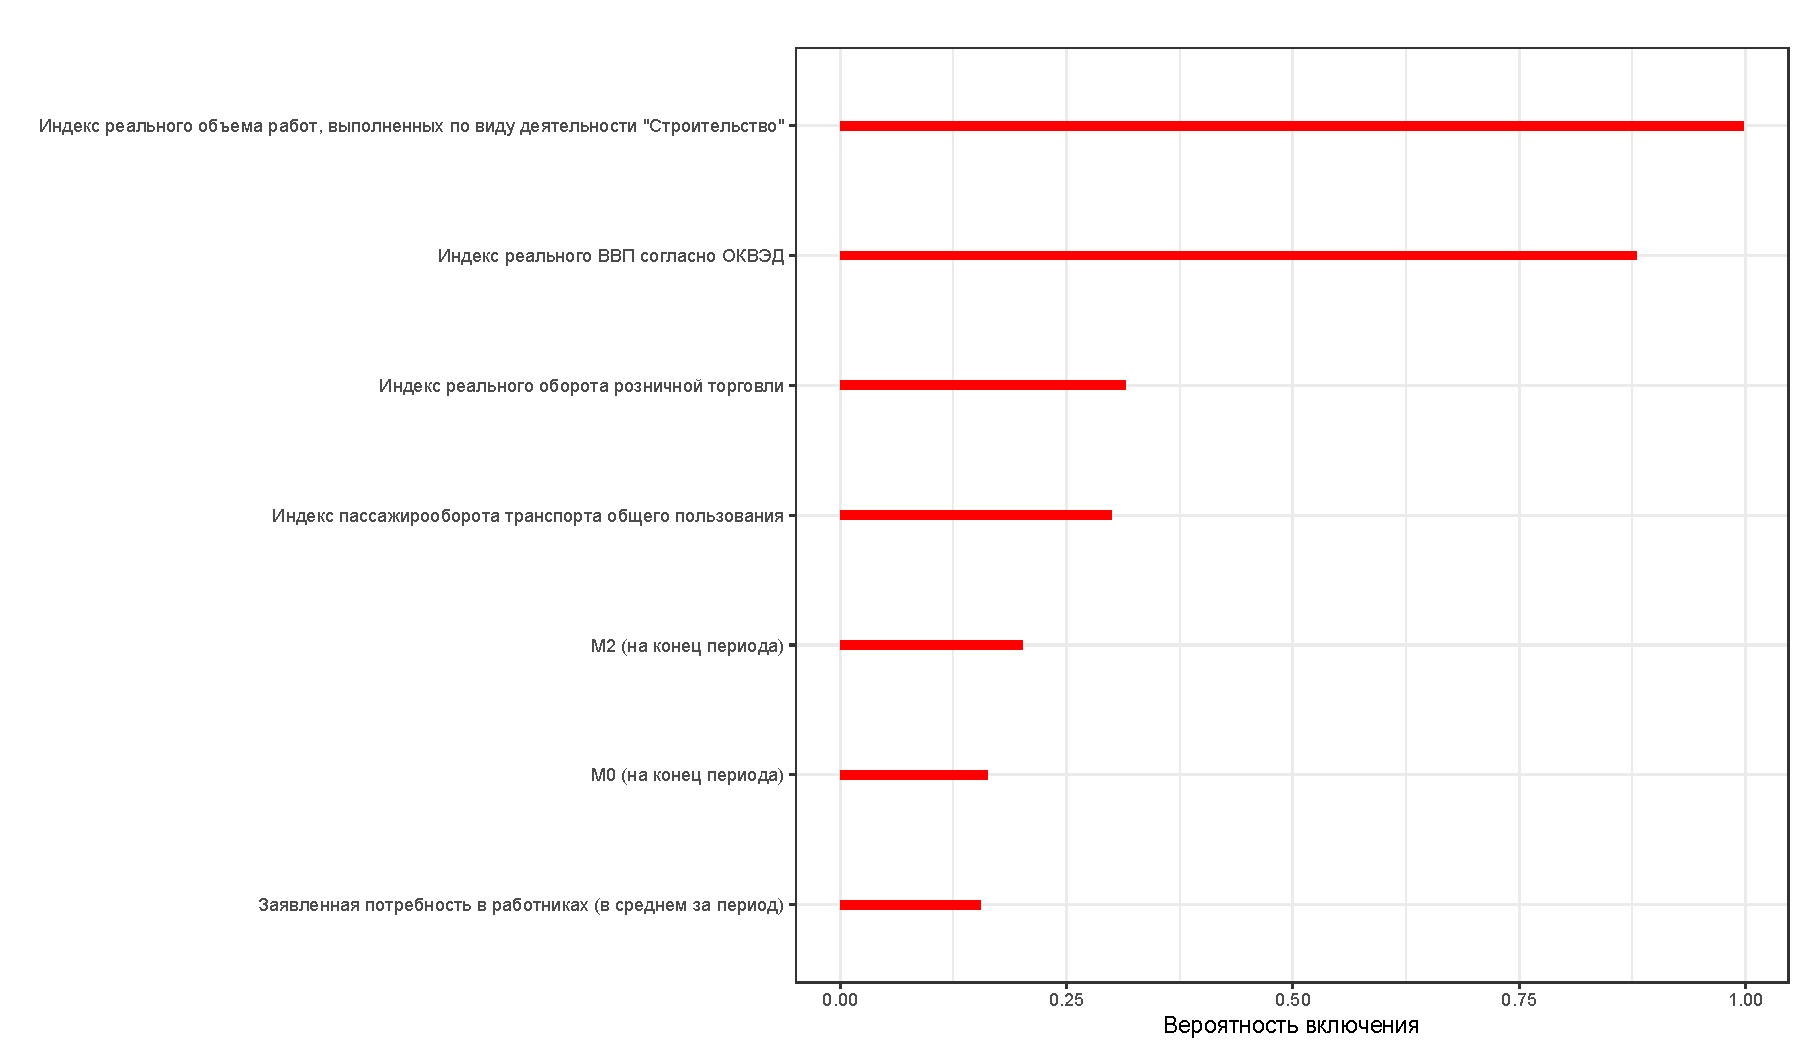
\includegraphics[width=\linewidth]{nzlollipop.pdf}
\end{figure*}
\end{frame} 

\begin{frame}
\frametitle{\insertsection} 
\framesubtitle{\insertsubsection}
\begin{figure*}
\caption{Значение коэффициентов LASSO для разных обучающих выборок}
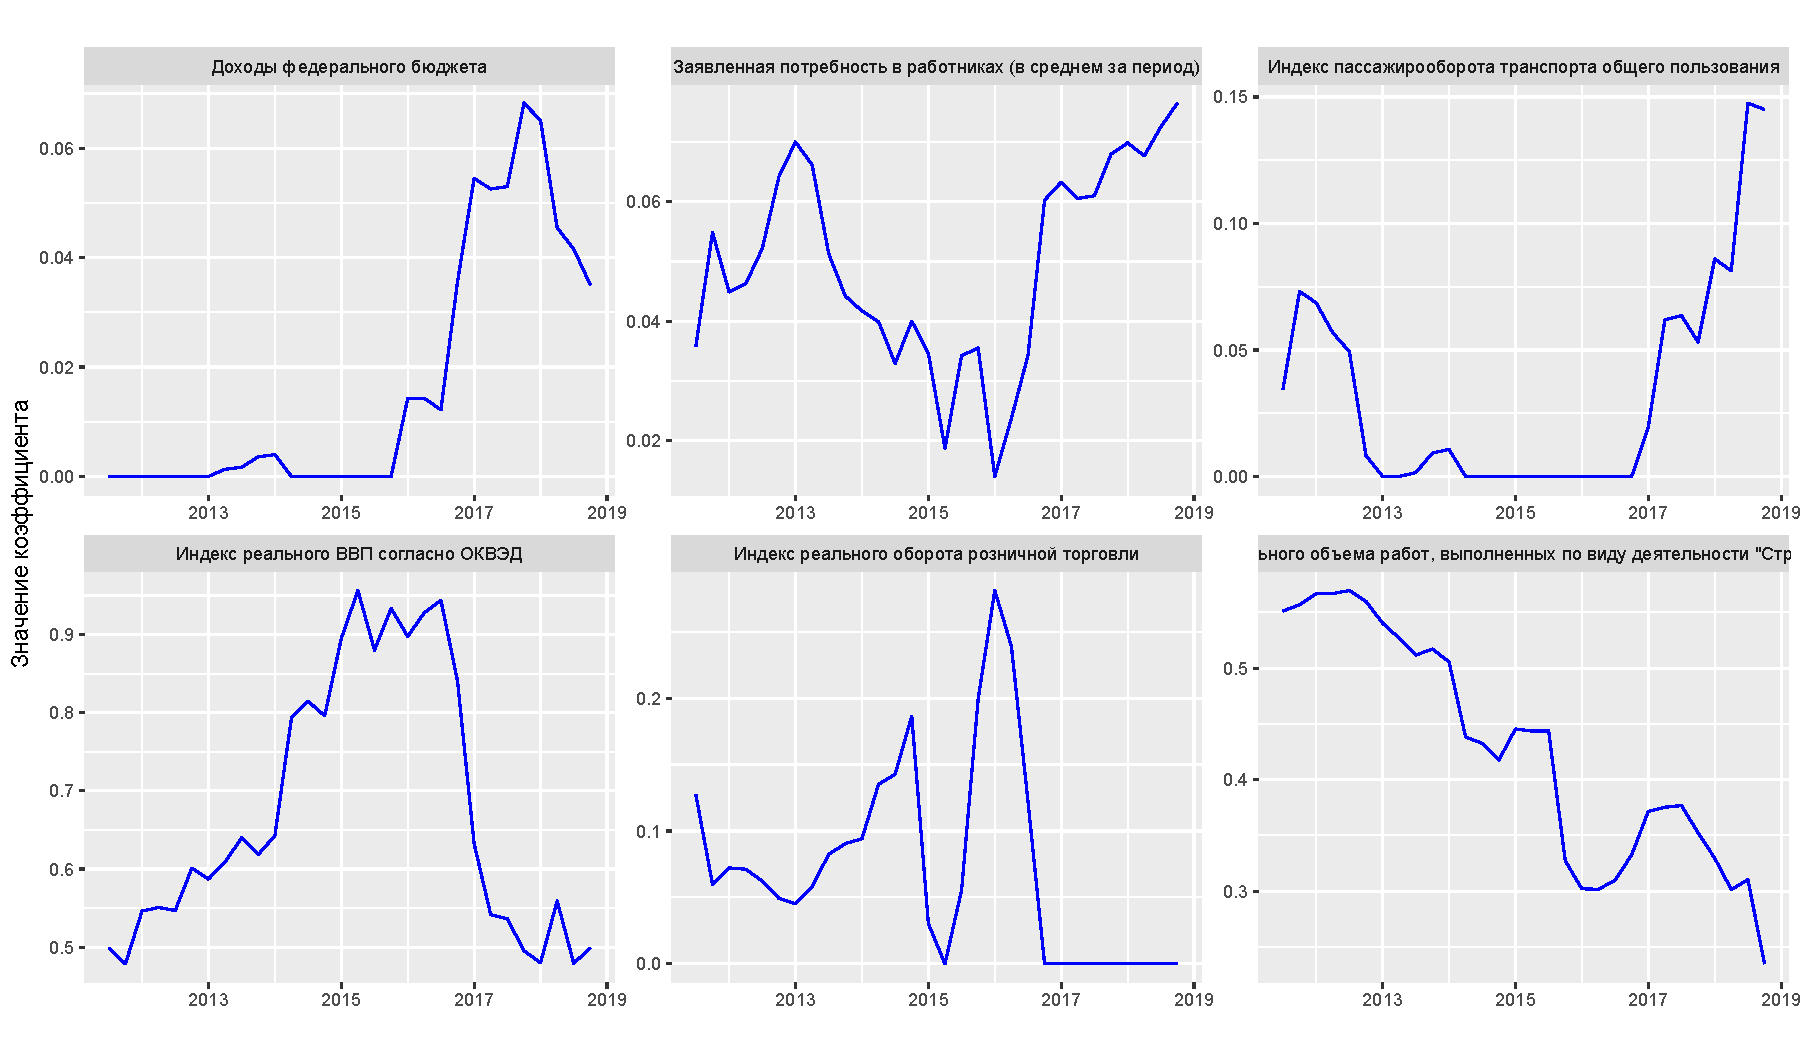
\includegraphics[width=\linewidth]{coef_plot.pdf}
\end{figure*}
\end{frame} 

\section{Итоги}
\begin{frame}
\frametitle{\insertsection} 
\framesubtitle{\insertsubsection} 
\begin{itemize}
    \item  Использование методов снижения размерности (LASSO, Post-LASSO, Ridge, случайный лес, пик-плато) позволяет в некоторых случаях достичь более высокого качество прогноза уровня инвестиций в России, чем использование традиционных моделей;
    \item Отбор дополнительных предикторов для традиционных моделей с помощью методов регуляризации тоже приводит к улучшению прогноза в случае модели q Тобина и неоклассической модели;
    \item Модель Adaptive LASSO, теоретически дающая состоятельные оценки коэффициентов, показала на практике худшие среди всех моделей результаты;
    \item Благодаря методам снижения размерности потенциально можно отбирать опережающие индикаторы уровня инвестиций в России (например, индекс объема строительства, заявленная потребность в работниках). 
\end{itemize}
   
    
\end{frame}





\begin{frame}[c, plain]
\begin{center}

{\LARGE Спасибо за внимание}

\bigskip

{\Large \inserttitle}

\bigskip

{\insertauthor} 

\bigskip

\bigskip\bigskip

{\large \insertdate}
\end{center}
\end{frame}



\begin{frame}[c, plain, shrink = 30]
  \frametitle{Источники}    
  \begin{thebibliography}{8}    
  \beamertemplatearticlebibitems

  \bibitem{ch1}
    Belloni, Alexandre and Chernozhukov, Victor
    \newblock High dimensional sparse econometric Моделs: An introduction.
    \newblock Springer, 2011
   \bibitem{ch2}
   Belloni, Alexandre, Victor Chernozhukov, and Christian Hansen. 
   \newblock Lasso methods for gaussian instrumental variables Модеls
   \newblock 2011
    \bibitem{bl}
    Barro, Robert J.  and Lee, Jong-Wha 
    \newblock Data Set for a Panel of 138 Countries
    \newblock 1994
    \bibitem{g}
     Candes, Emmanuel, and Terence Tao. 
    \newblock The Dantzig selector: Statistical estimation when p is much larger than n.
    \newblock The Annals of Statistics 35.6 (2007): 2313--2351.
    \bibitem{f}
     Akaike, Hirotugu.
    \newblock A new look at the statistical Модель identification.
    \newblock IEEE transactions on automatic control 19.6 (1974): 716--723.
    \bibitem{s}
    Единый архив экономических и социологических данных, статистические ряды
    \newblock http://sophist.hse.ru/hse/nindex.shtml
    \bibitem{z}
    Zou, Hui
    \newblock The adaptive lasso and its oracle properties
    \newblock Journal of the American statistical association (2006): 1418--1429
  \end{thebibliography}
\end{frame}

\section{Приложение}
 \begin{frame}
 \frametitle{\insertsection} 
\framesubtitle{\insertsubsection}
\begin{table}[ht]
\centering
\begin{tabular}{lrrrrrr}
  \hline
Модель & 1 & 2 & 3 & 4 & 5 & 6 \\ 
  \hline
Adaptive LASSO & 0.45 & 0.60 & 0.73 & 0.63 & 0.82 & 0.97 \\ 
  Boosting & 0.60 & 0.75 & \alert{0.63} & 0.60 & 0.77 & 0.86 \\ 
  Elastic Net & 0.42 & 0.57 & 0.67 & 0.59 & 0.76 & 0.92 \\ 
  LASSO & \alert{0.41} & \alert{0.54} & 0.65 & \alert{0.55} & \alert{0.71} & \alert{0.85} \\ 
  LASSO+PC & 0.70 & 0.99 & 1.14 & 1.19 & 1.49 & 1.79 \\ 
  LASSO+VAR & 1.20 & 1.38 & 1.28 & 1.14 & 1.25 & 1.40 \\ 
  Post LASSO & 0.49 & 0.74 & 0.79 & 0.77 & 0.90 & 1.18 \\ 
  Random Forest & 0.75 & 0.93 & 0.80 & 0.73 & 0.91 & 1.00 \\ 
  Ridge & 0.44 & 0.60 & 0.69 & 0.64 & 0.82 & 0.99 \\ 
  Spike and Slab & 0.56 & 0.65 & 0.72 & 0.61 & 0.76 & 0.83 \\ 
   \hline
\end{tabular}
\end{table}
\end{frame}

 \begin{frame}
 \frametitle{\insertsection} 
\framesubtitle{\insertsubsection}
\begin{table}[ht]
\centering
\begin{tabular}{lrrrrrr}
  \hline
Модель & 7 & 8 & 9 & 10 & 11 & 12 \\ 
  \hline
Adaptive LASSO & 1.05 & 0.93 & 1.08 & 1.18 & 1.27 & 1.15 \\ 
  Boosting & \alert{0.72} &\alert{ 0.73} & \alert{0.81} & \alert{0.84} & \alert{0.72} & \alert{0.74} \\ 
  Elastic Net & 0.96 & 0.86 & 0.97 & 1.09 & 1.13 & 1.02 \\ 
  LASSO & 0.90 & 0.79 & 0.90 & 1.00 & 1.06 & 0.95 \\ 
  LASSO+PC & 1.86 & 1.94 & 2.13 & 2.31 & 2.35 & 2.47 \\ 
  LASSO+VAR & 1.41 & 1.34 & 1.50 & 1.67 & 1.78 & 1.78 \\ 
  Post LASSO & 1.15 & 1.14 & 1.21 & 1.42 & 1.40 & 1.39 \\ 
  Random Forest & 0.85 & 0.83 & 0.94 & 0.94 & 0.81 & 0.82 \\ 
  Ridge & 1.02 & 0.94 & 1.06 & 1.18 & 1.20 & 1.11 \\ 
  Spike and Slab & 0.88 & 0.77 & 0.89 & 0.92 & 0.97 & 0.85 \\ 
   \hline
\end{tabular}
\end{table}
\end{frame}

\begin{frame}
\frametitle{\insertsection} 
\framesubtitle{\insertsubsection}
\begin{figure*}
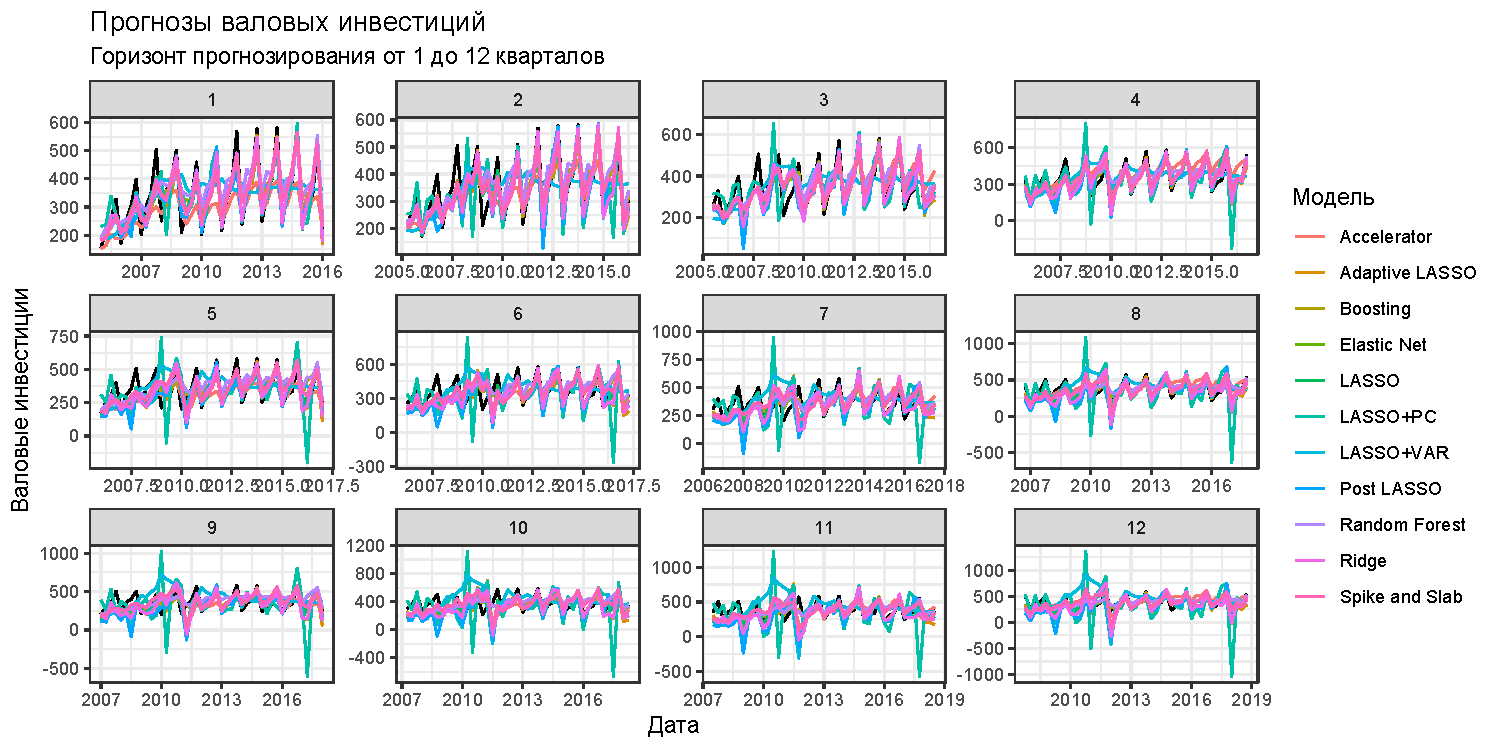
\includegraphics[width=\linewidth]{bad_outall.pdf}
\end{figure*}
\end{frame} 
 
 
 \begin{frame}
\frametitle{\insertsection} 
\framesubtitle{\insertsubsection}
\begin{figure*}
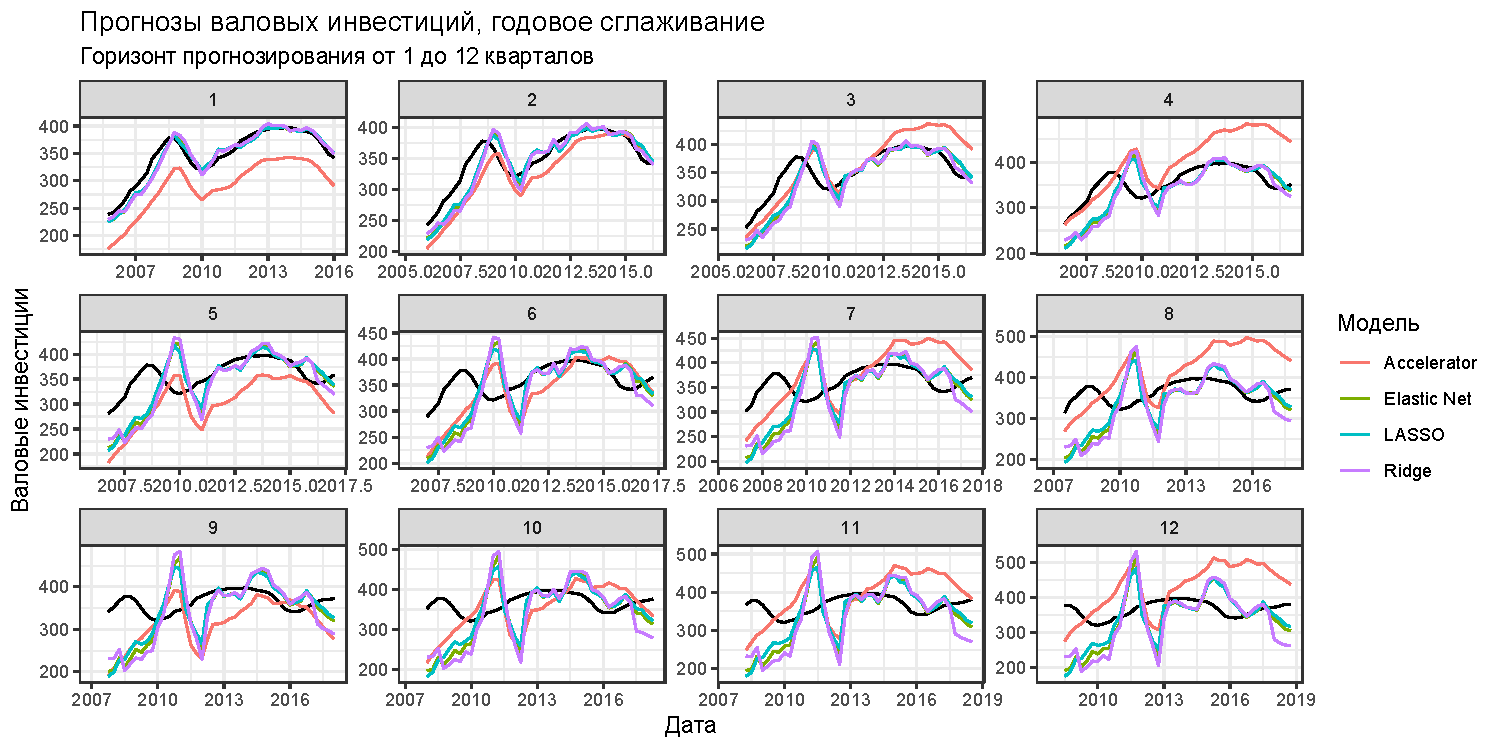
\includegraphics[width=\linewidth]{smooth1.pdf}
\end{figure*}
\end{frame} 


 \begin{frame}
\frametitle{\insertsection} 
\framesubtitle{\insertsubsection} 
\begin{figure*}
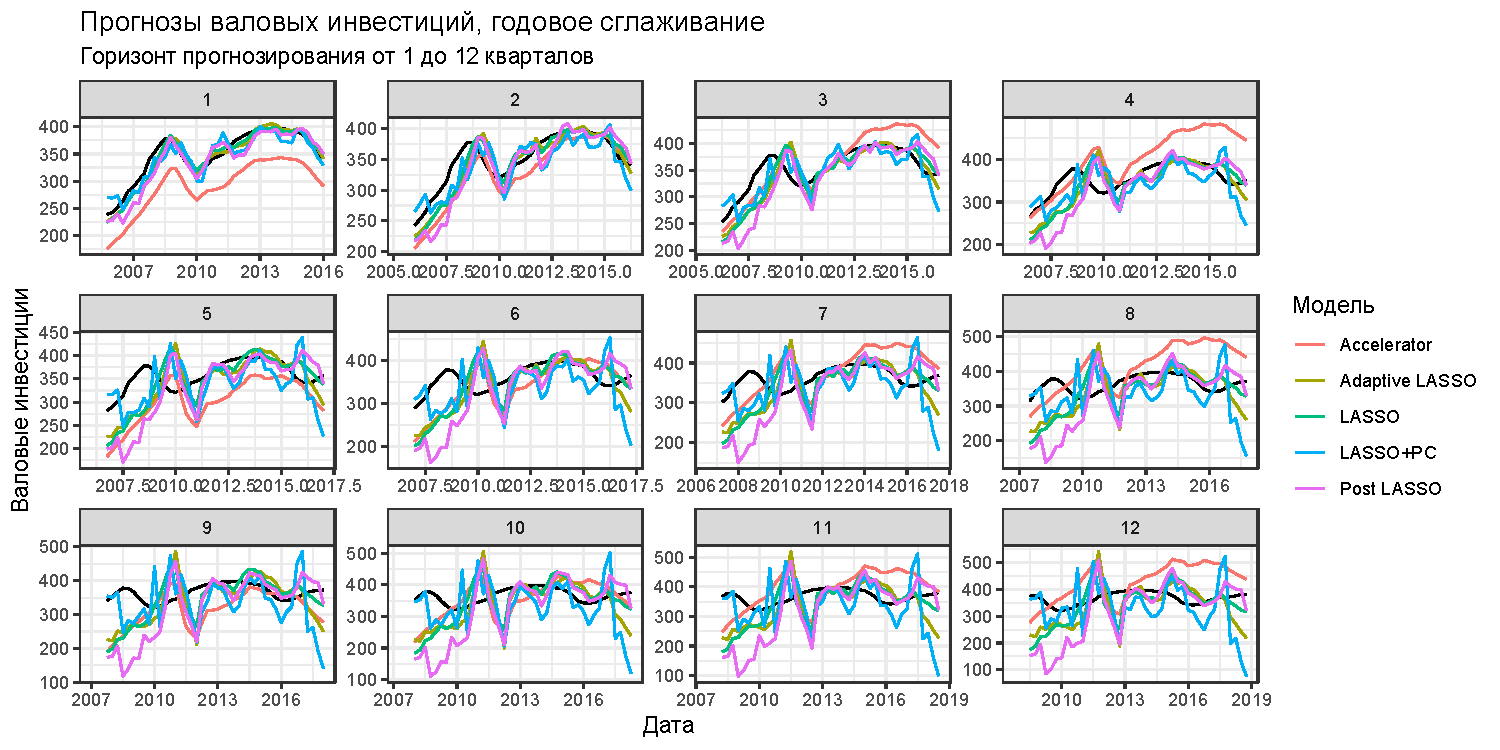
\includegraphics[width=\linewidth]{smooth2.pdf}
\end{figure*}
\end{frame} 

 \begin{frame}
\frametitle{\insertsection} 
\framesubtitle{\insertsubsection}
\begin{figure*}
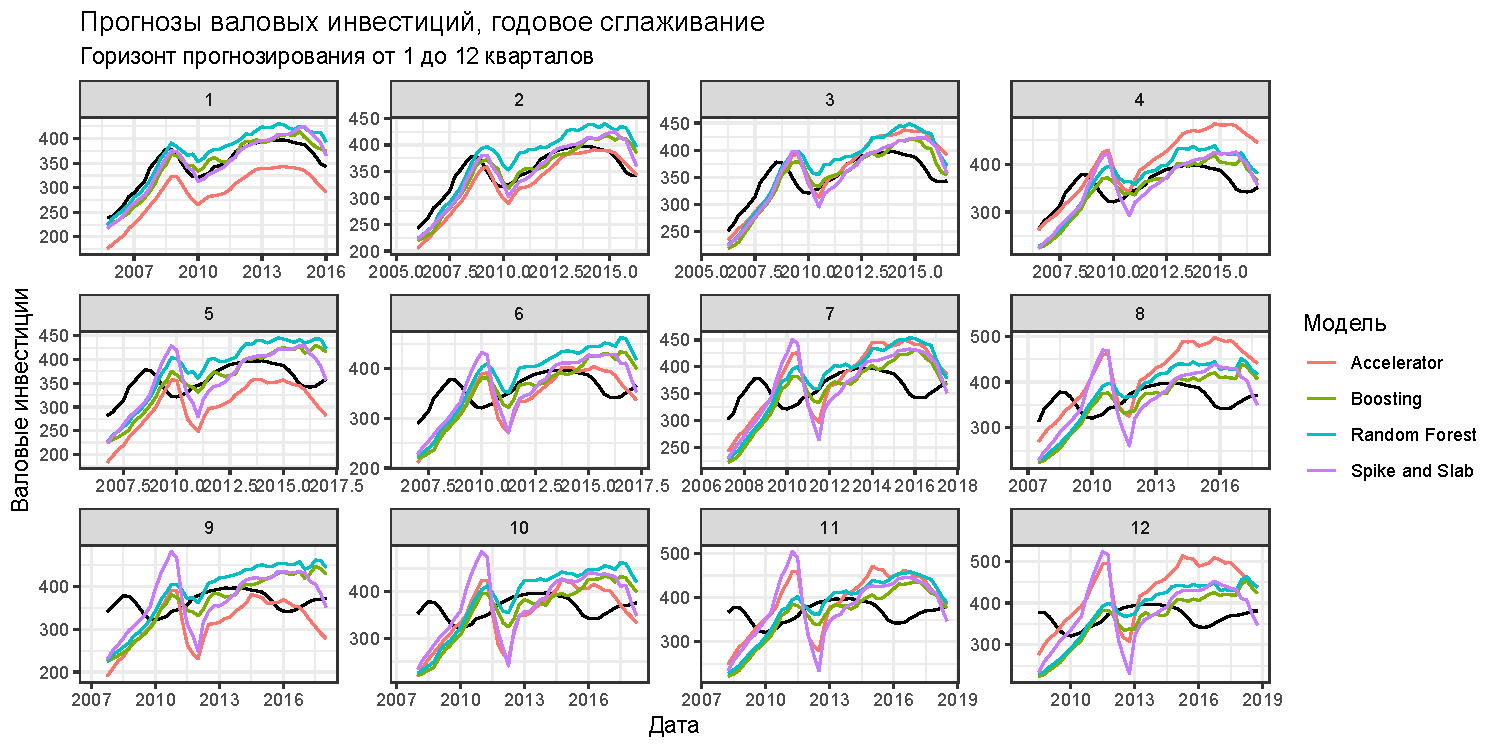
\includegraphics[width=\linewidth]{smooth3.pdf}
\end{figure*}
\end{frame} 

 \begin{frame}
\frametitle{\insertsection} 
\framesubtitle{\insertsubsection}
\begin{figure*}
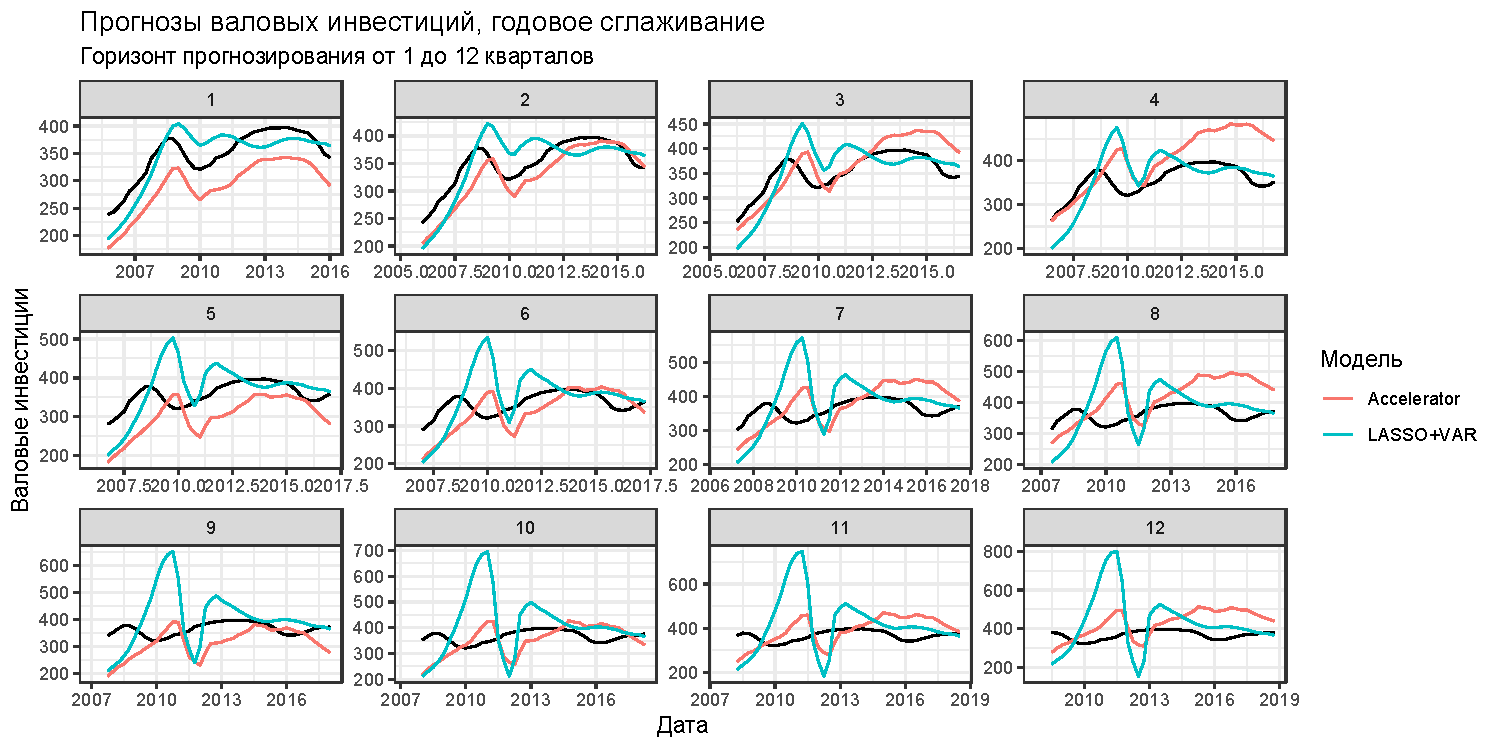
\includegraphics[width=\linewidth]{smooth4.pdf}
\end{figure*}
\end{frame} 


 \begin{frame}
\frametitle{\insertsection} 
\framesubtitle{\insertsubsection}
\begin{figure*}
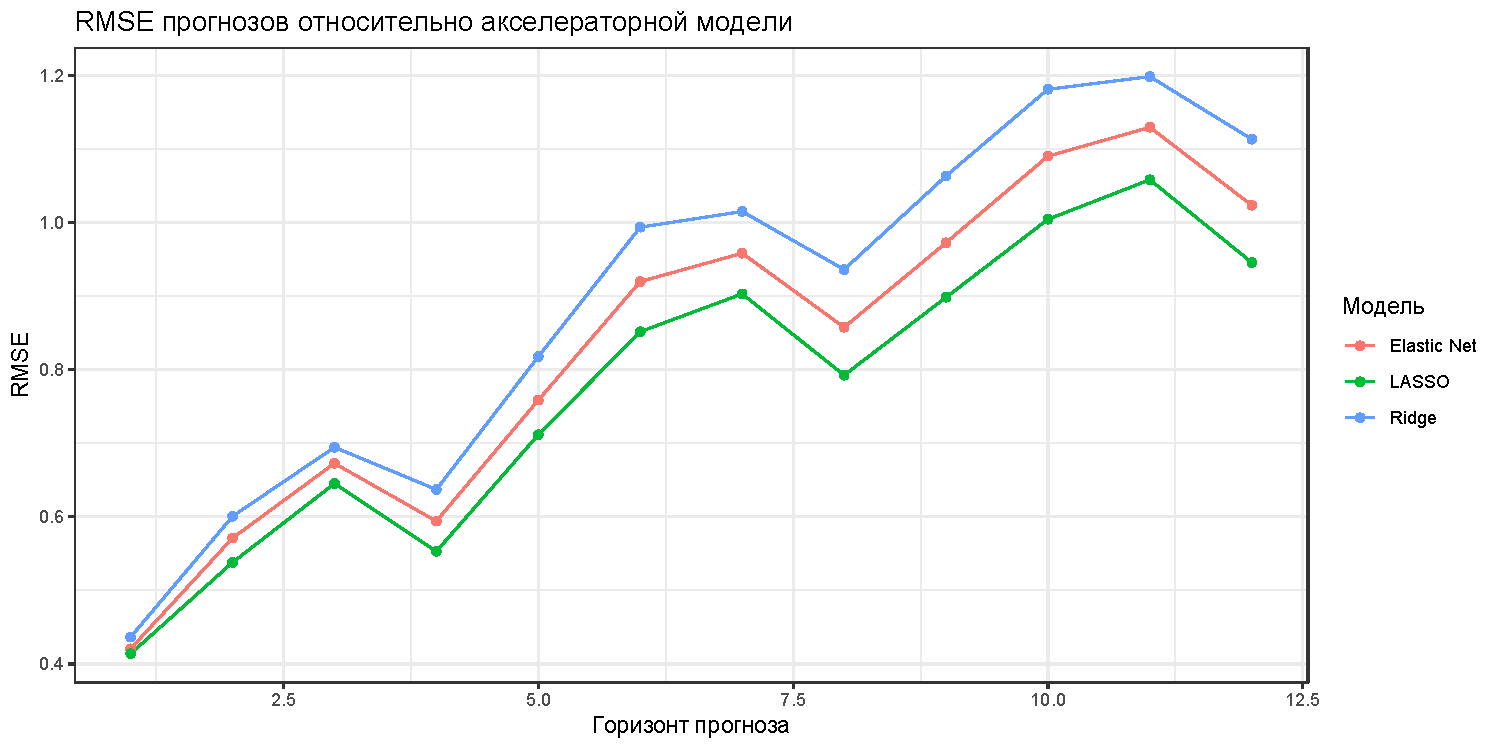
\includegraphics[width=\linewidth]{rmse1.pdf}
\end{figure*}
\end{frame} 


 \begin{frame}
\frametitle{\insertsection} 
\framesubtitle{\insertsubsection}
\begin{figure*}
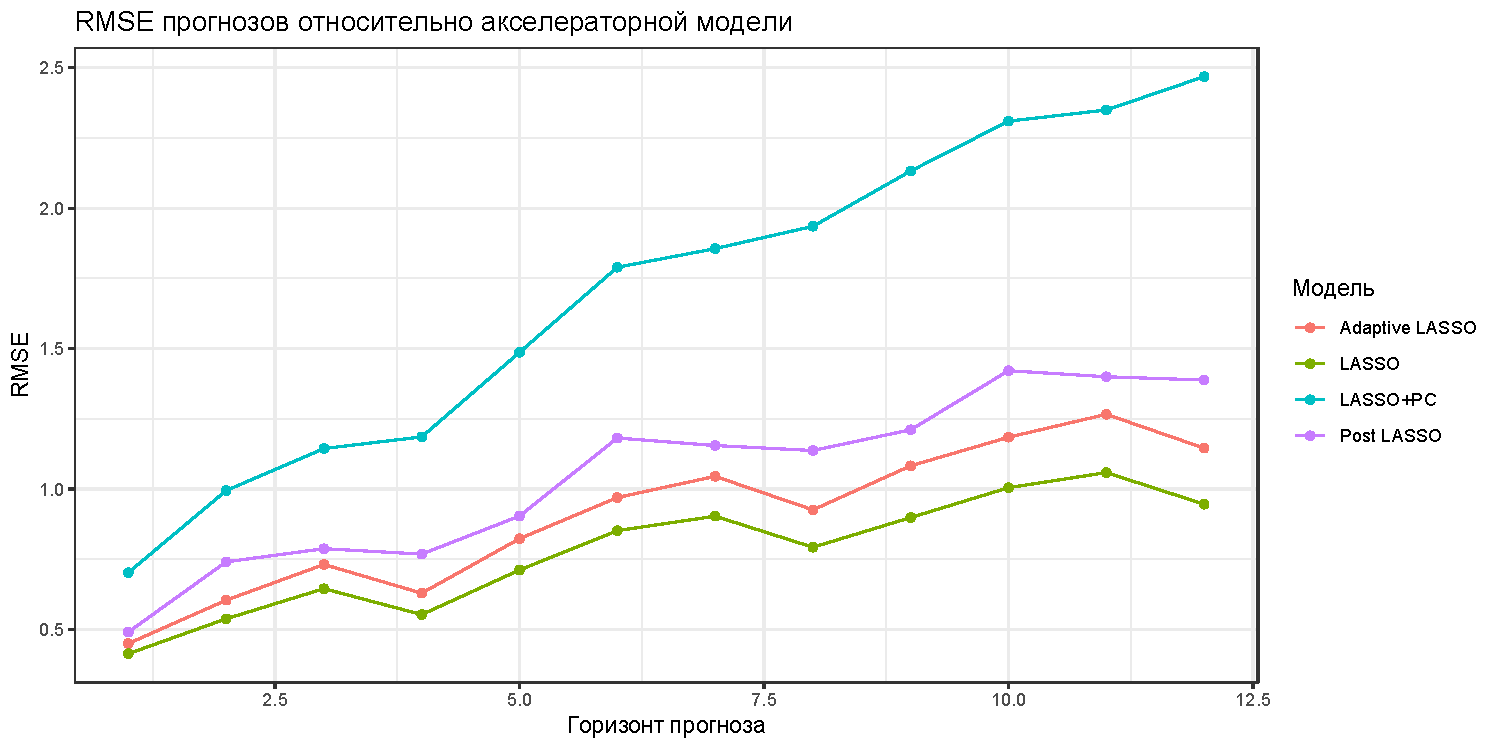
\includegraphics[width=\linewidth]{rmse2.pdf}
\end{figure*}
\end{frame} 


 \begin{frame}
\frametitle{\insertsection} 
\framesubtitle{\insertsubsection}
\begin{figure*}
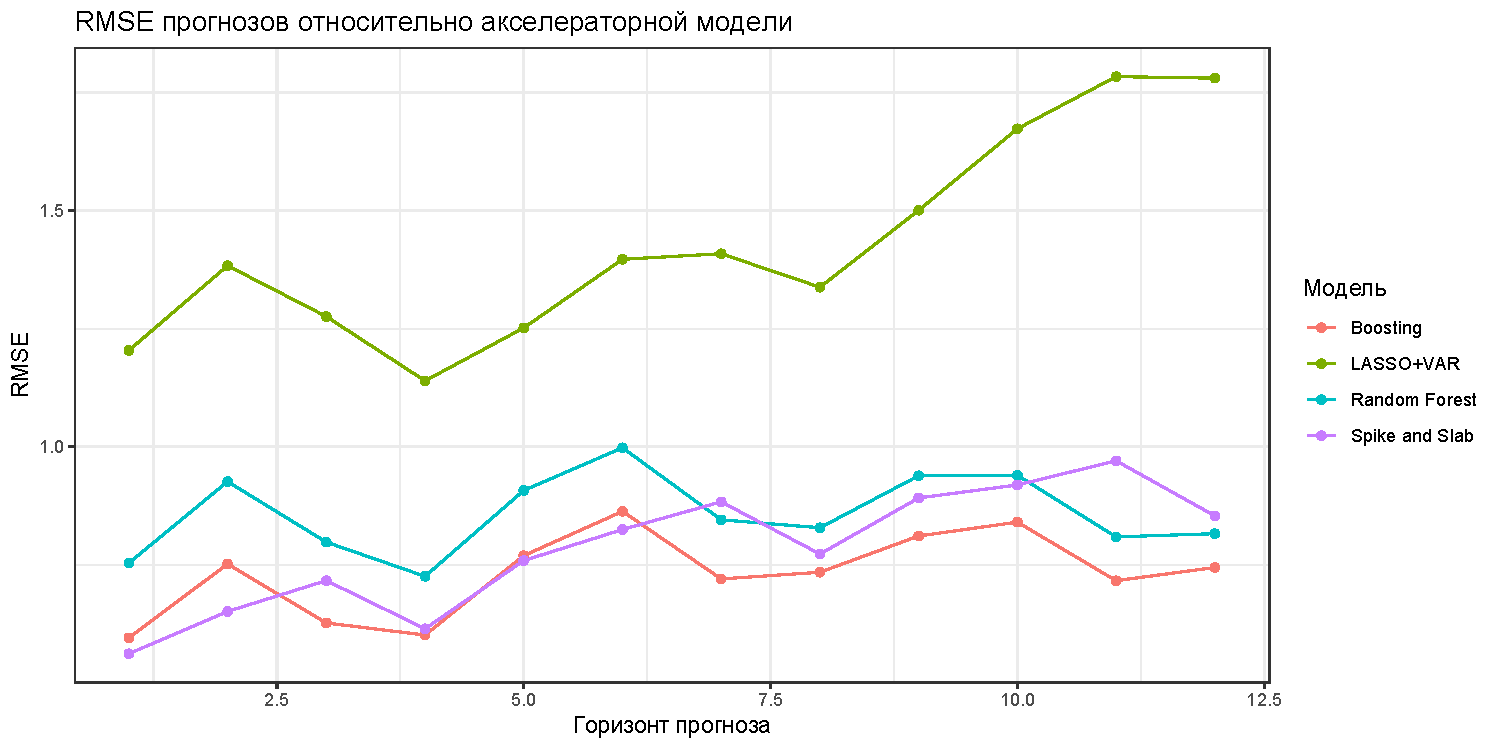
\includegraphics[width=\linewidth]{rmse3.pdf}
\end{figure*}
\end{frame} 


 \begin{frame}
\frametitle{\insertsection} 
\framesubtitle{\insertsubsection}
\begin{figure*}
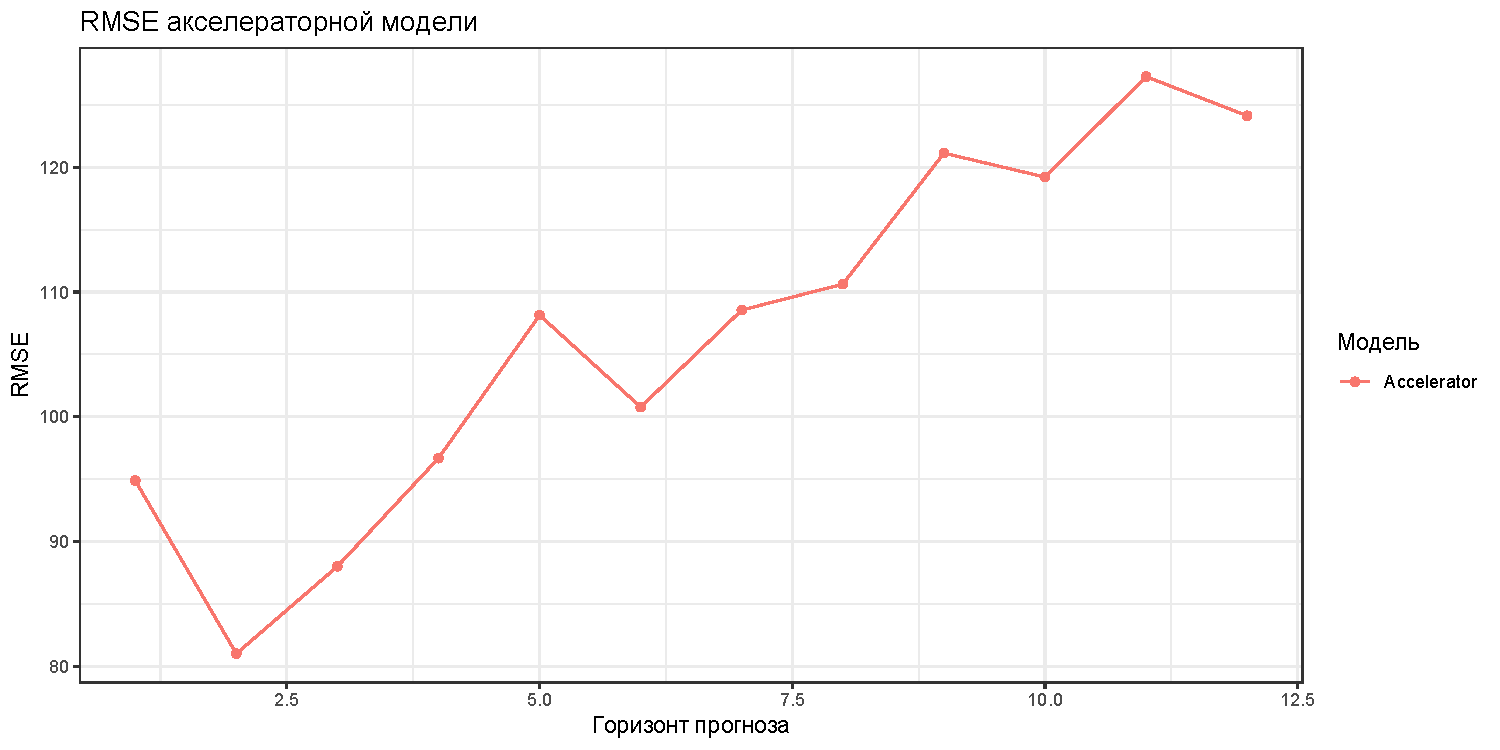
\includegraphics[width=\linewidth]{rmse4.pdf}
\end{figure*}
\end{frame} 


 \begin{frame}
\frametitle{\insertsection} 
\framesubtitle{\insertsubsection}
\begin{figure*}
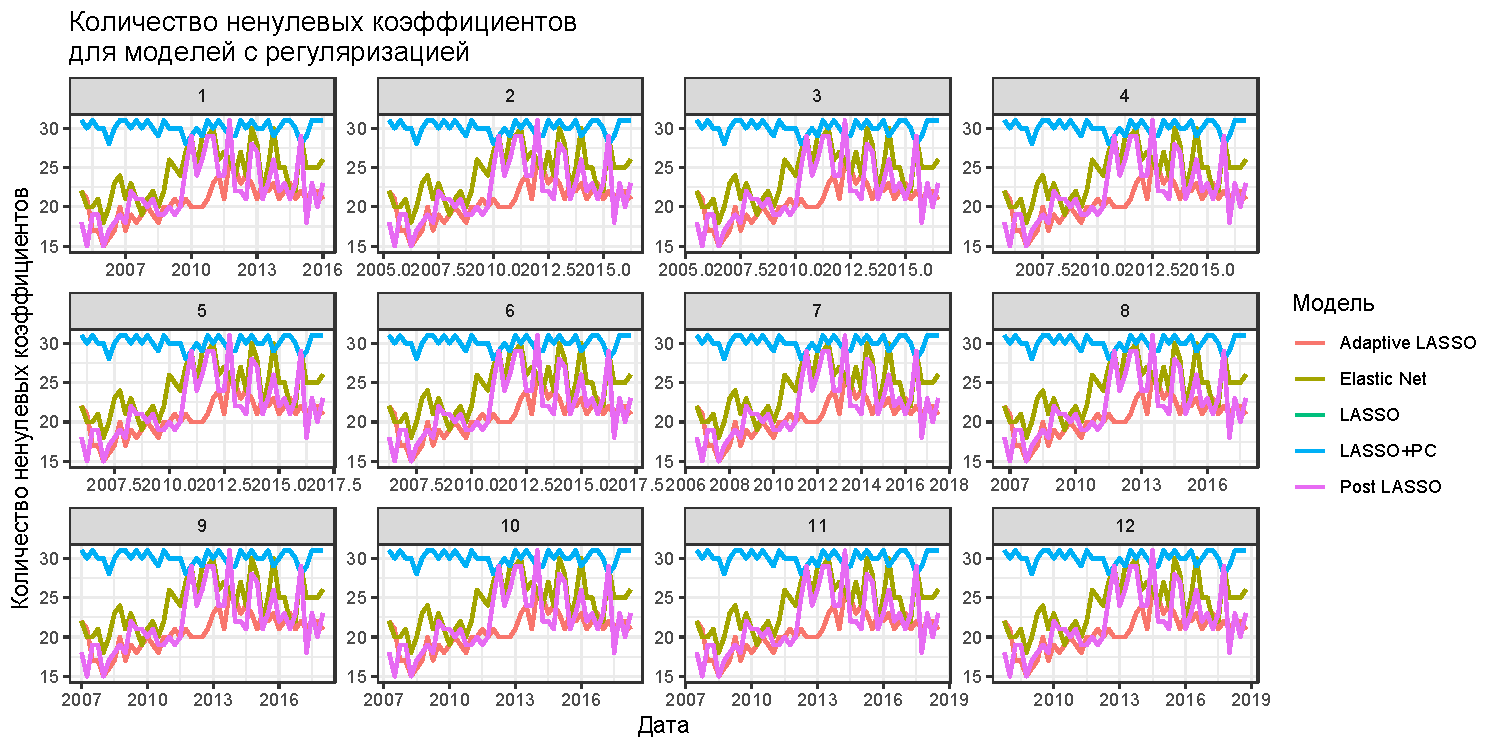
\includegraphics[width=\linewidth]{nonzerotime.pdf}
\end{figure*}
\end{frame} 


 \begin{frame}
\frametitle{\insertsection} 
\framesubtitle{\insertsubsection}
\begin{figure*}
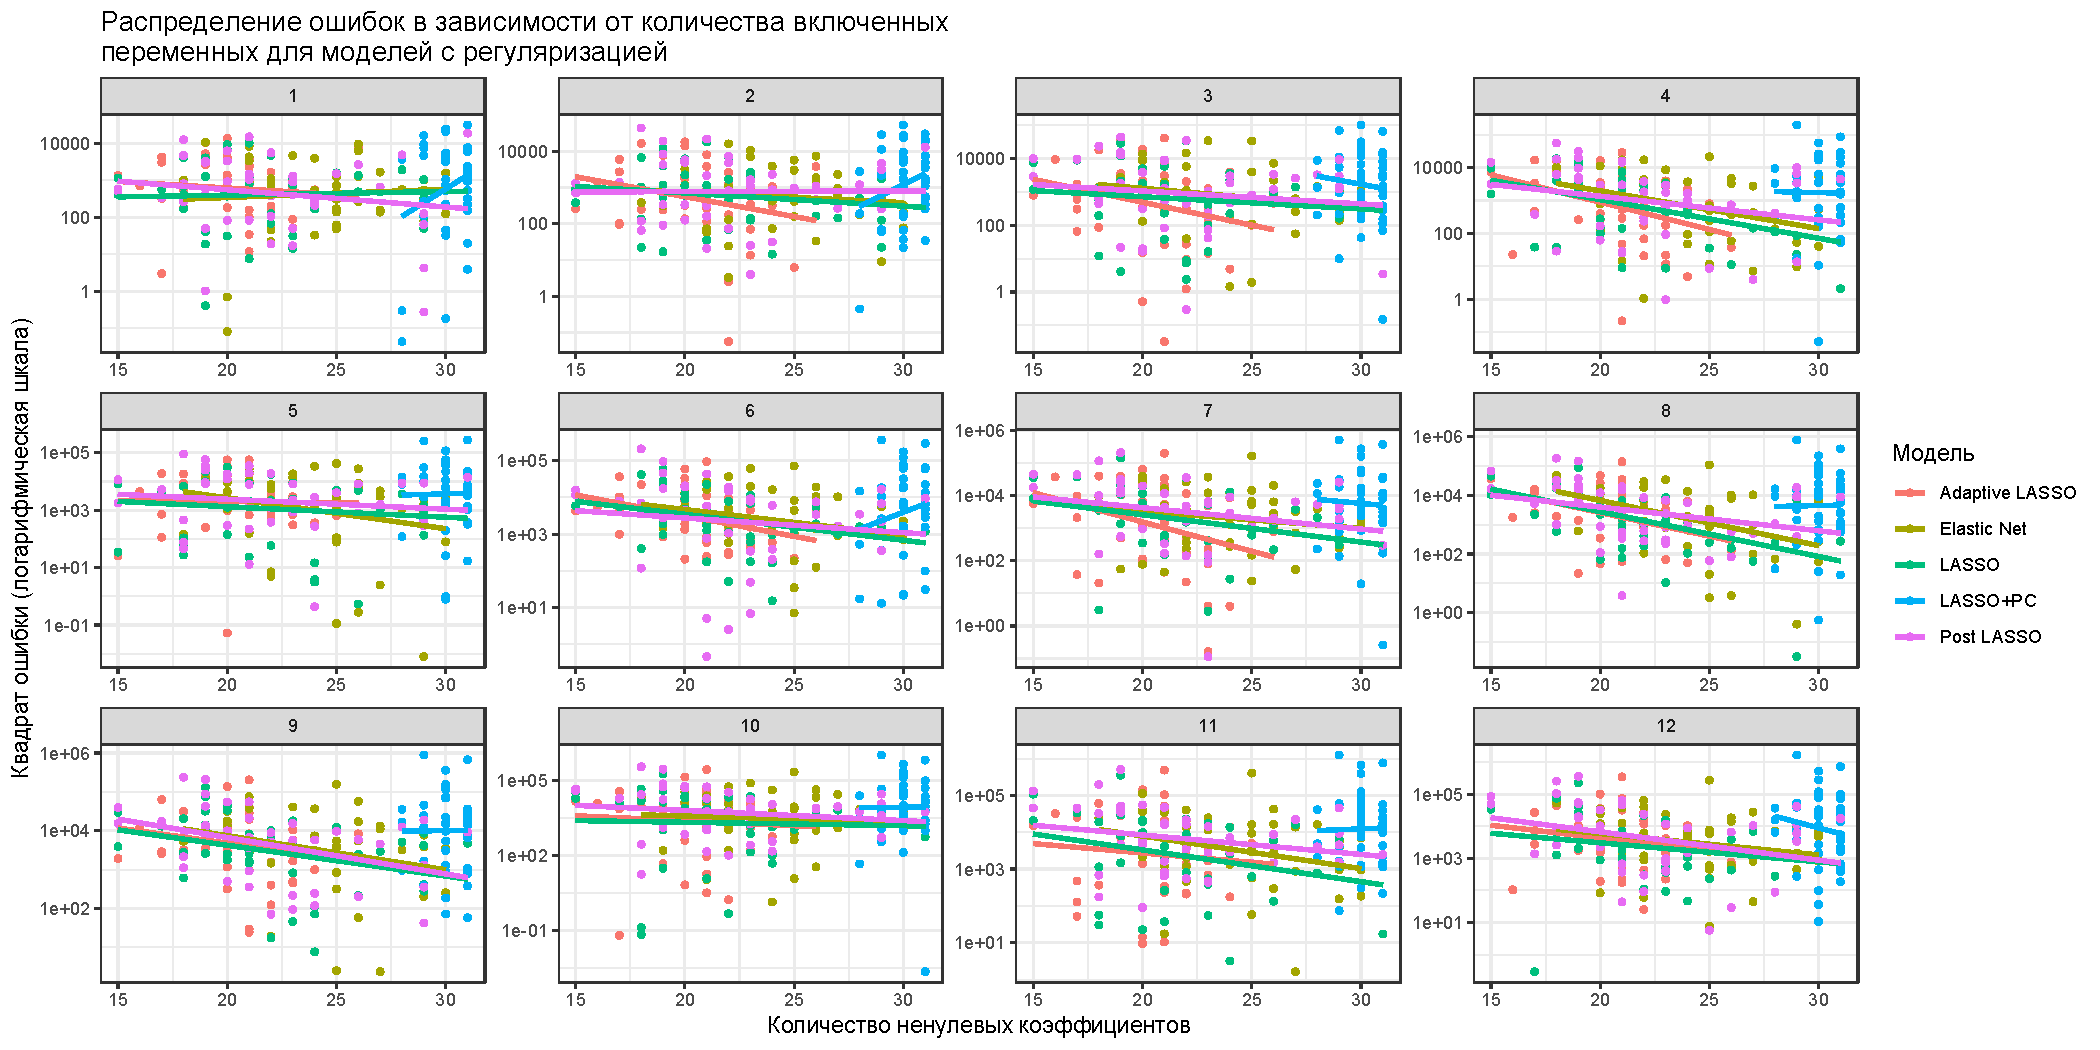
\includegraphics[width=\linewidth]{nonzeroerror.pdf}
\end{figure*}
\end{frame} 

 \begin{frame}
\frametitle{\insertsection} 
\framesubtitle{\insertsubsection} 
\begin{figure*}
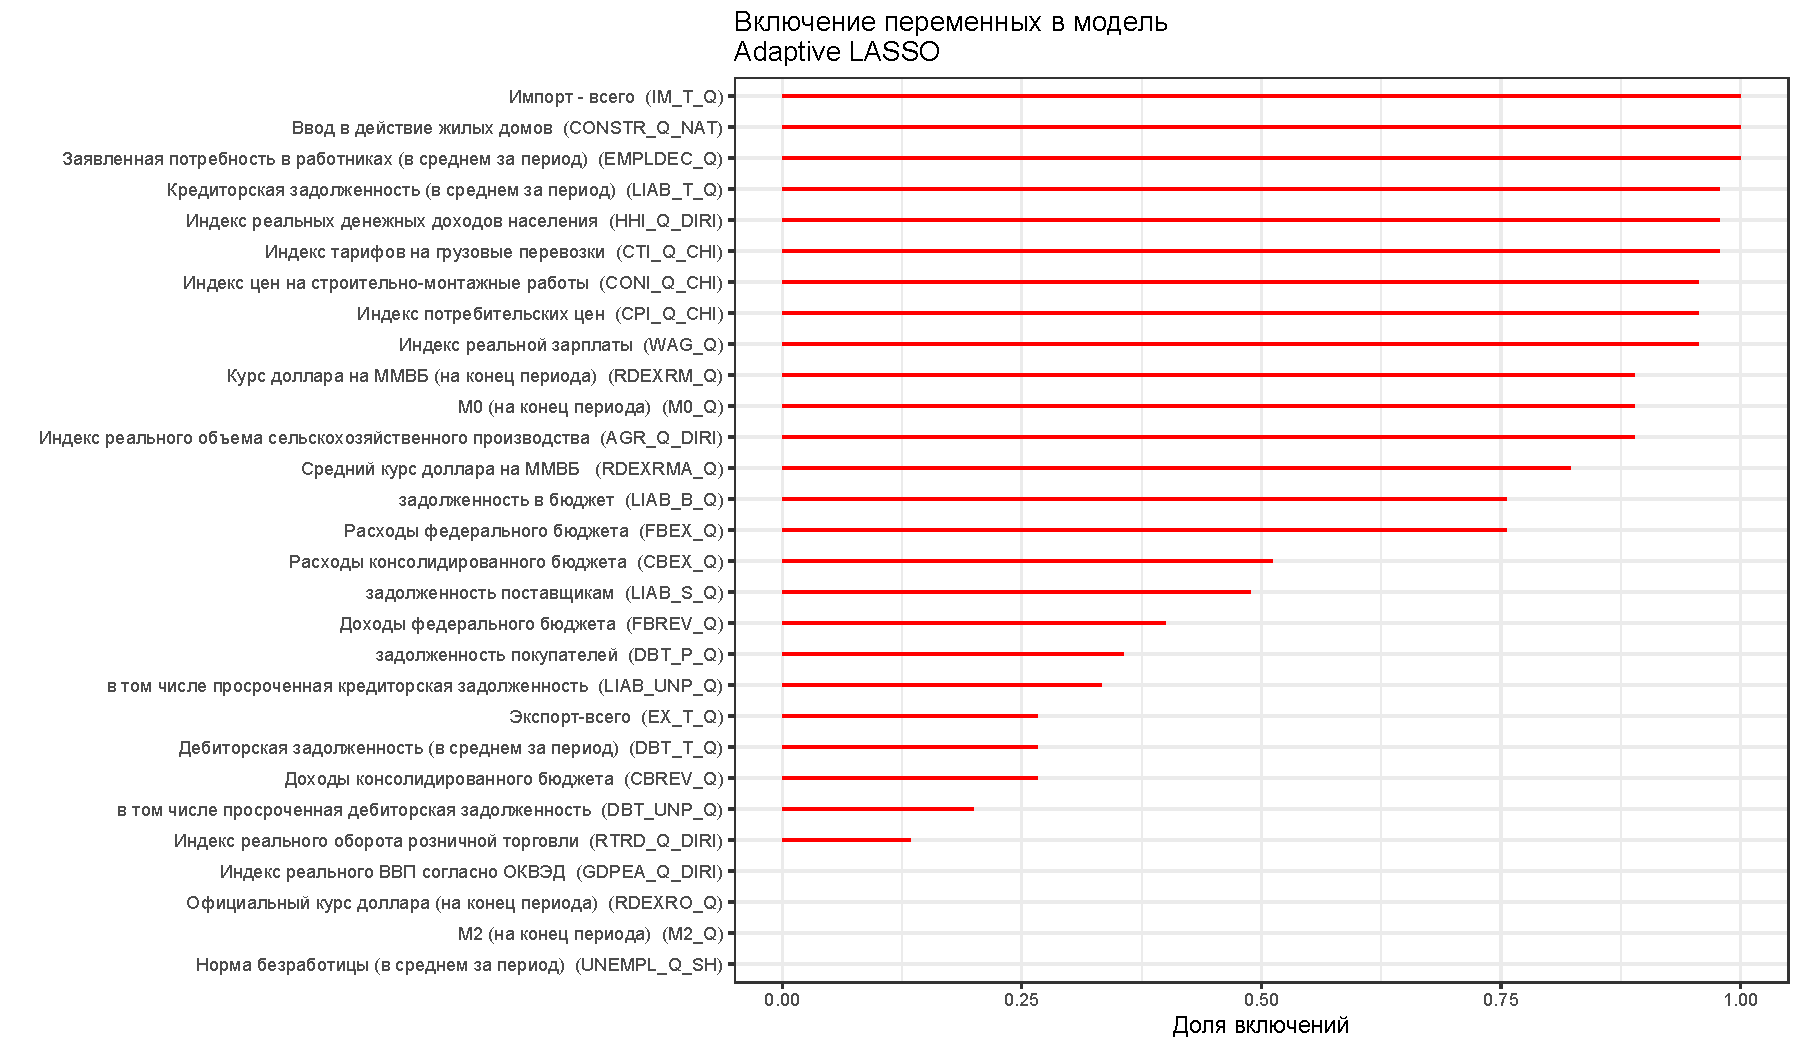
\includegraphics[width=\linewidth]{nzlollipop1.pdf}
\end{figure*}
\end{frame} 

 \begin{frame}
\frametitle{\insertsection} 
\framesubtitle{\insertsubsection}
\begin{figure*}
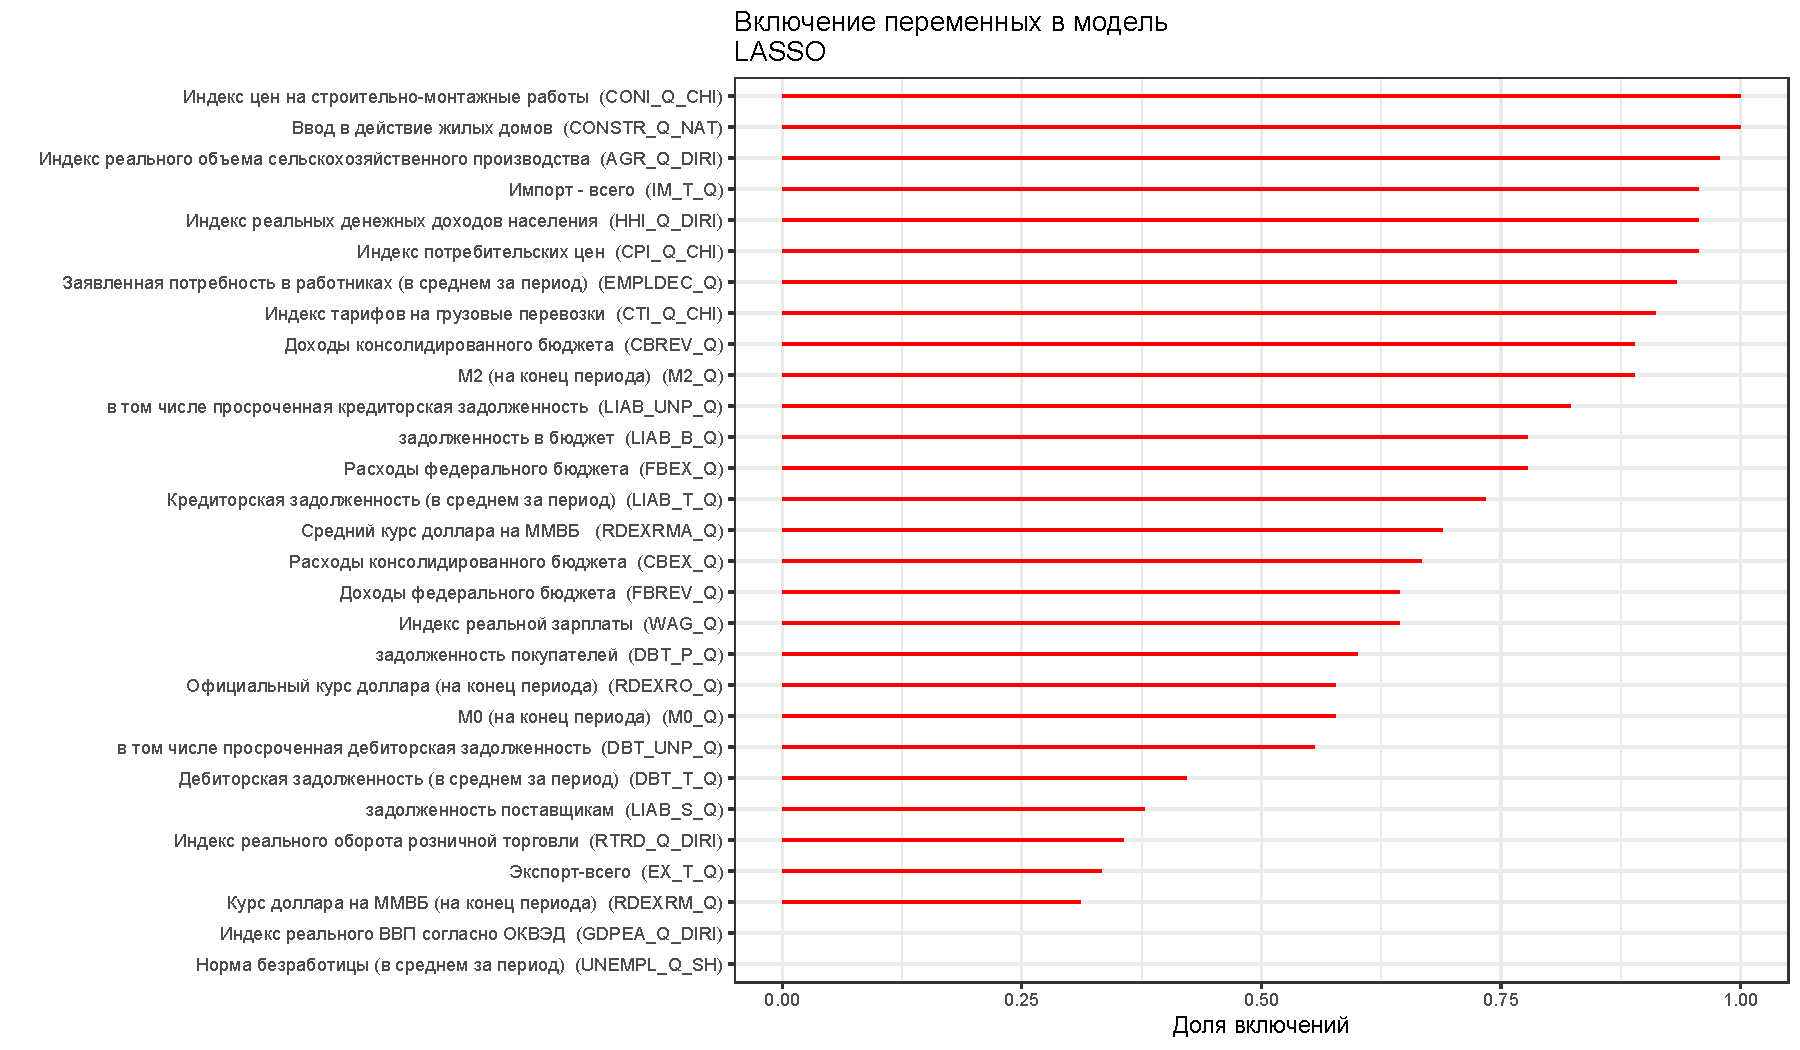
\includegraphics[width=\linewidth]{nzlollipop2.pdf}
\end{figure*}
\end{frame} 

\end{document}